\documentclass{cs202}
% \usepackage{ctex}
% \documentclass[\zihao{1}]{cs202}
% =============================================
% Part 0 信息
% =============================================

\mathsetup{
    % 学生姓名
    studentA = {张辰星},
    % 学号
    studentA-id = {20202297},
    % 学生姓名
    studentB = {包梵轩},
    % 学号
    studentB-id = {2022****},
      % 学生姓名
    studentC = {沈奕俊},
    % 学号
    studentC-id = {2022****},
    % 学生姓名
    % 院系
    institution = {数理学院数学系},
    % 专业年级
    discipline = {信息与计算科学专业 2020 级},
    % 日期
    date = {\today},
}

\begin{document}
\zihao{-4}

% =============================================
% Part 1  封面
% =============================================

\makecover


% =============================================
% Part 2 主文档
% =============================================

\section{系统需求分析}

\subsection{系统目的和意义}

\subsubsection{系统目的:}
进行毕业设计需求分析、完善毕设管理流程。
在此基础上进行整体技术架构设计、功能设计和数据库设计,
并对系统进行实现。
旨在构建一个高效、易用的毕业设计管理系统,为数理学院教务工作提供便利。

\subsubsection{系统意义:}
计算机技术与网络技术日新月异的发展,
推动了信息技术在社会各个领域的广泛应用,
也为教育带来了不可估量的影响,
而且人们的上网时空已经不受限制,
随着移动平台的普及,
手机、iPad等产品越来越多地被使用。
尤其在教育领域,目前,我国许多高校的各项管理工作都在向信息化建设迈进,
以校园网为平台的“数字化”校园建设情况已经成为衡量高校信息化建设水平的一个标志。
而作为高校重点管理工作的毕业设计管理,其管理水平是否先进对学校办学质量具有举足轻重的影响。
尤其在校园网络的基础上,
建立高校毕业设计管理模式和信息化管理平台,
开发具有自身院校特点的毕业设计管理系统非常重要。


\subsection{功能模块划分}

\subsubsection{登录窗口}
在此毕业设计管理系统中,
我们设计了管理员端、教师端以及学生端三个端,
通过在登陆界面输入不同的账户名可以分别登入各个端。

\subsubsection{管理员端}
在管理员端中,我们预计开设五个模块,分别为:
参数设置、课题审核、选题操作、选题结果以及修改密码模块。
分别用于实现对专业、教师提交题目截止时间、管理员审核题目截止时间、
学生第一次选题开始时间、学生第一次选题截止时间、管理员第一次匹配截止时间
学生第二次选题截止时间、管理员第二次匹配截止时间进行设置;
查看课题的编号、名称、指导老师、所属专业年级以及审核情况,
对课题进行审核操作;
设置提前批选题的学号以及题号,
查看第一第二次选题分配情况,
导出选题匹配结果以及选题失败同学名单;
查看学生选题的课题编号、学号、姓名、课题名称、指导老师以及学年的信息,
按年份筛选、搜索课题和导出选题结果表格;
重置教师和学生的密码的功能。

\subsubsection{教师端}
在教师端中,拟开设四个模块,分别为:
课题提交、选题列表、选题结果和修改密码模块。
分别用于输入课题的各项基本信息;
查看提交的课题的信息并进行修改删除等操作;
查看学生的选题结果信息,包括学生姓名学号专业班级联系方式;
最后提供了教师更新密码的窗口。

\subsubsection{学生端}
在管理员端中,我们预计开设五个模块,分别为:
选题规则、选题操作、预选志愿、选题结果以及修改密码模块。
学生登入后就会自动跳转到选题规则页面,让学生们了解选题的具体规则,
减少出现因不熟悉规则而导致选题出现的错误;
选题操作界面可以查看课题的内容信息,仅包含课题的名称、编号以及类别信息,
防止学生们选老师而不是选课题;
在预选志愿界面,学生可以查看自己预选的第一到第四志愿,以及对应课题的信息,
方便学生进行检查确认;
在选题结果模块中,学生可以查看自己最后选择到的课题的课题编号、名称信息,
并且可以查看自己课题的指导老师;
修改密码界面提供了平台供同学们更新自己的密码。


\subsection{系统开发环境}

\begin{itemize}
    \item 前端:
          \begin{itemize}
              \item node.js
              \item React
              \item Redux
              \item JavaScript
          \end{itemize}
    \item 后端:
          \begin{itemize}
              \item Python
              \item FastAPI
              \item SQLAlchemy
              \item Alembic
          \end{itemize}
\end{itemize}


\section{系统概念结构设计}

\subsection{登录界面}
\begin{itemize}
    \item 管理员账户
    \item 教师账户
    \item 学生账户
\end{itemize}

\subsection{管理员端}
\begin{itemize}
    \item 参数设置
    \item 课题审核
    \item 选课操作
    \item 选课结果
    \item 修改密码
\end{itemize}

\subsection{教师端}
\begin{itemize}
    \item 课题提交
    \item 选课列表
    \item 选课结果
    \item 修改密码
\end{itemize}

\subsection{学生端}
\begin{itemize}
    \item 选课规则
    \item 选课操作
    \item 预选志愿
    \item 选课结果
    \item 修改密码
\end{itemize}


% =============================================
% Part 3  系统逻辑结构设计
% =============================================



\section{系统逻辑结构设计}

\subsection{关系模型}
\begin{figure}[h]
    \centering
    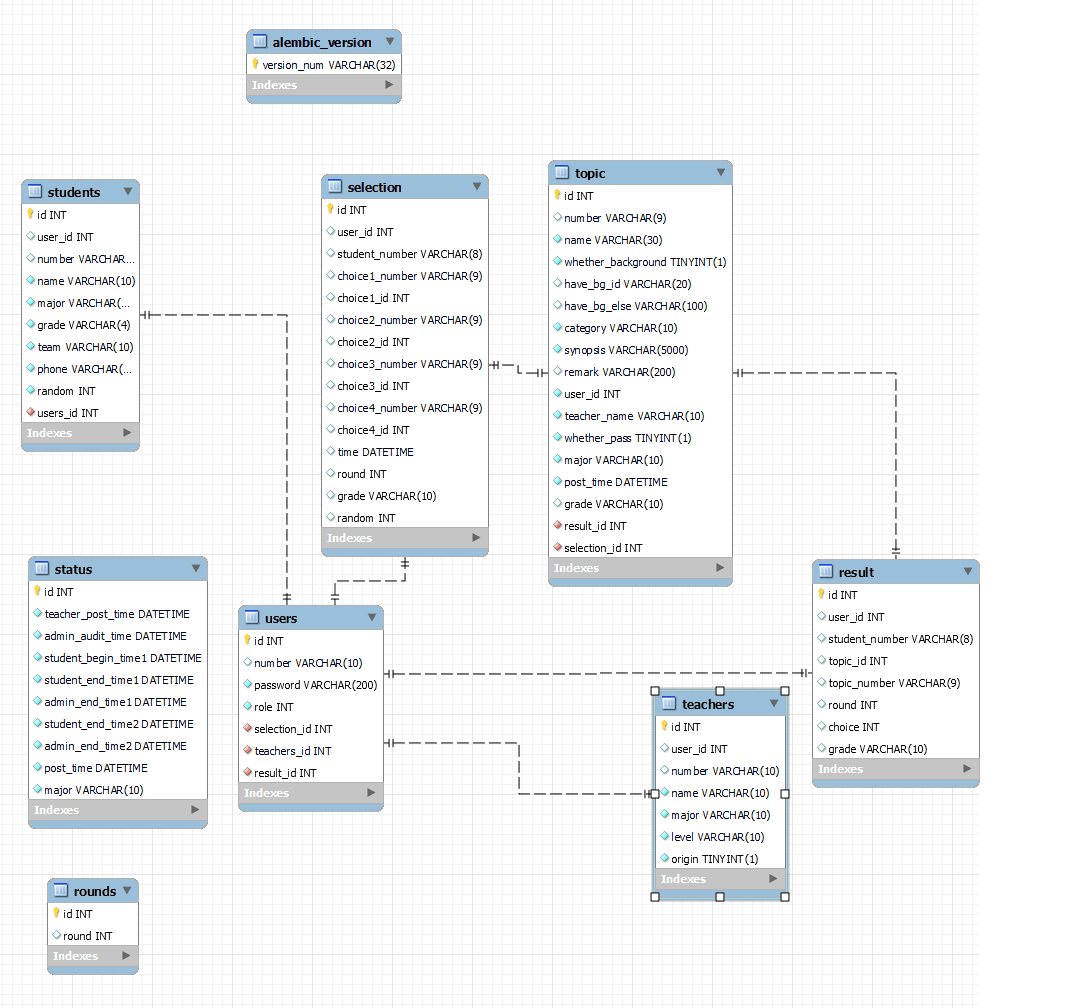
\includegraphics[width=0.7\textwidth]{关系模型.png}
    \caption{关系模型}
    \label{fig:ER}
\end{figure}

\clearpage

\subsection{数据库设计}



\begin{table}[ht]
    \centering
    \caption{users表}
    \begin{tabular}{|c|c|}
        \hline
        列名          & 备注     \\
        \hline
        id          & 自增主键id \\
        \hline
        number(int) & 用户id   \\
        \hline
        password    & 用户密码   \\
        \hline
        role(int)   & 用户权限   \\
        \hline
    \end{tabular}
    
    \label{tab:users}
\end{table}


\begin{table}[ht]
    \centering
    \caption{teachers表}
    \begin{tabular}{|c|c|}
        \hline
        列属性           & 备注               \\
        \hline
        id            & 自增主键id           \\
        \hline
        user\_id(int) & users外键id        \\
        \hline
        number(str)   & 教师工号             \\
        \hline
        name(str)     & 教师姓名             \\
        \hline
        major(str)    & 教师专业             \\
        \hline
        level(str)    & 教师职称             \\
        \hline
        origin(bool)  & 教师是否来自校外,默认false \\
        \hline
    \end{tabular}
    
    \label{tab:teachers}
\end{table}


\begin{table}[ht]
    \centering
    \caption{students表}
    \begin{tabular}{|c|c|}
        \hline
        列属性           & 备注        \\
        \hline
        id            & 自增主键id    \\
        \hline
        user\_id(int) & users外键id \\
        \hline
        number(str)   & 学生学号      \\
        \hline
        name(str)     & 学生姓名      \\
        \hline
        major(str)    & 学生专业      \\
        \hline
        grade(str)    & 年级        \\
        \hline
        team(str)     & 班级        \\
        \hline
        phone(str)    & 电话号码      \\
        \hline
        random(int)   & 随机数       \\
        \hline
    \end{tabular}
    
    \label{tab:students}
\end{table}

\clearpage

\begin{table}[ht]
    \centering
    \caption{status表(储存各种时间相关的数据)管理员设置}
    \begin{tabular}{|c|c|}
        \hline
        列属性                             & 备注                       \\
        \hline
        id                              & 自增主键id                   \\
        \hline
        teacher\_post\_time(datatime)   & 教师提交题目截止时间/管理员审核题目开始时间   \\
        \hline
        admin\_audit\_time(datatime)    & 管理员审核题目截止时间/学生浏览题目开始时间   \\
        \hline
        student\_begin\_time1(datatime) & 学生第一次选题开始时间/学生浏览题目结束时间   \\
        \hline
        student\_end\_time1(datatime)   & 学生第一次选题截止时间/管理员第一次匹配开始时间 \\
        \hline
        admin\_end\_time1(datatime)     & 管理员第一次匹配截止时间/学生第二次选题开始时间 \\
        \hline
        student\_end\_time2(datatime)   & 学生第二次选题截止时间/管理员第二次匹配开始时间 \\
        \hline
        admin\_end\_time2               & 管理员第二次匹配截止时间             \\
        \hline
        post\_time(datatime)            & 当前提交时间                   \\
        \hline
        major(str)                      & 设置适用的专业                  \\
        \hline
    \end{tabular}
    
    \label{tab:status}
\end{table}

\begin{table}[ht]
    \centering
    \caption{topic表}
    \begin{tabular}{|c|c|}
        \hline
        列属性                       & 备注                    \\
        \hline
        id                        & 自增主键id                \\
        \hline
        number                    & 课题编号                  \\
        \hline
        name(str)                 & 课题名称                  \\
        \hline
        whether\_background(bool) & 是否有项目背景,default=false \\
        \hline
        have\_bg\_id(str)         & 有背景的项目id              \\
        \hline
        have\_bg\_else(str)       & 有背景的项目补充              \\
        \hline
        category(str)             & 课题性质(类别)              \\
        \hline
        synopsis(str)             & 课题简介                  \\
        \hline
        remark(str)               & 备注                    \\
        \hline
        user\_id(int)             & 教师ID                  \\
        \hline
        teacher\_name(str)        & 指导教师名称                \\
        \hline
        whether\_pass(bool)       & 是否审核通过,default=false  \\
        \hline
        major(str)                & 课题适用专业                \\
        \hline
        topic\_time(datatime)     & 课题提交时间                \\
        \hline
    \end{tabular}
   
    \label{tab:topic}
\end{table}

\clearpage

\begin{table}[ht]
    \centering
    \caption{selection表}
    \begin{tabular}{|c|c|}
        \hline
        列属性                  & 备注       \\
        \hline
        id                   & 自增主键id   \\
        \hline
        user\_id(int)        & 学生ID     \\
        \hline
        student\_number(str) & 学生学号     \\
        \hline
        choice1\_number(str) & 第一志愿课题编号 \\
        \hline
        choice1\_id(int)     & 第一志愿id   \\
        \hline
        choice2\_number(str) & 第二志愿课题编号 \\
        \hline
        choice2\_id(int)     & 第二志愿id   \\
        \hline
        choice3\_number(str) & 第三志愿课题编号 \\
        \hline
        choice3\_id(int)     & 第三志愿id   \\
        \hline
        choice4\_number(str) & 第四志愿课题编号 \\
        \hline
        choice4\_id(int)     & 第四志愿id   \\
        \hline
        time(DateTime)       & 选题时间     \\
        \hline
        round(str)           & 第几轮选题    \\
        \hline
    \end{tabular}
    
    \label{tab:selection}
\end{table}

\begin{table}[ht]
    \centering
    \caption{result表}
    \begin{tabular}{|c|c|}
        \hline
        列属性                  & 备注     \\
        \hline
        id                   & 自增主键id \\
        \hline
        user\_id(int)        & 学生ID   \\
        \hline
        student\_number(str) & 学生学号   \\
        \hline
        topic\_id(int)       & 课题ID   \\
        \hline
        topic\_number(str)   & 课题编号   \\
        \hline
        round(str)           & 选中轮次   \\
        \hline
        choice(str)          & 选中志愿   \\
        \hline
    \end{tabular}
    
    \label{tab:result}
\end{table}

\clearpage


% =============================================
% Part 4 系统实现
% =============================================

\section{系统实现}

\subsection{系统管理员端}

\subsubsection{参数设置:}
在参数设置模块中,管理员可以对专业、教师提交题目截止时间、管理员审核题目截止时间、
学生第一次选题开始时间、学生第一次选题截止时间、管理员第一次匹配截止时间
学生第二次选题截止时间、管理员第二次匹配截止时间进行设置。
\begin{figure}[ht] % "h" 表示图片放置在文本所在位置,也可以使用其他选项
    \centering
    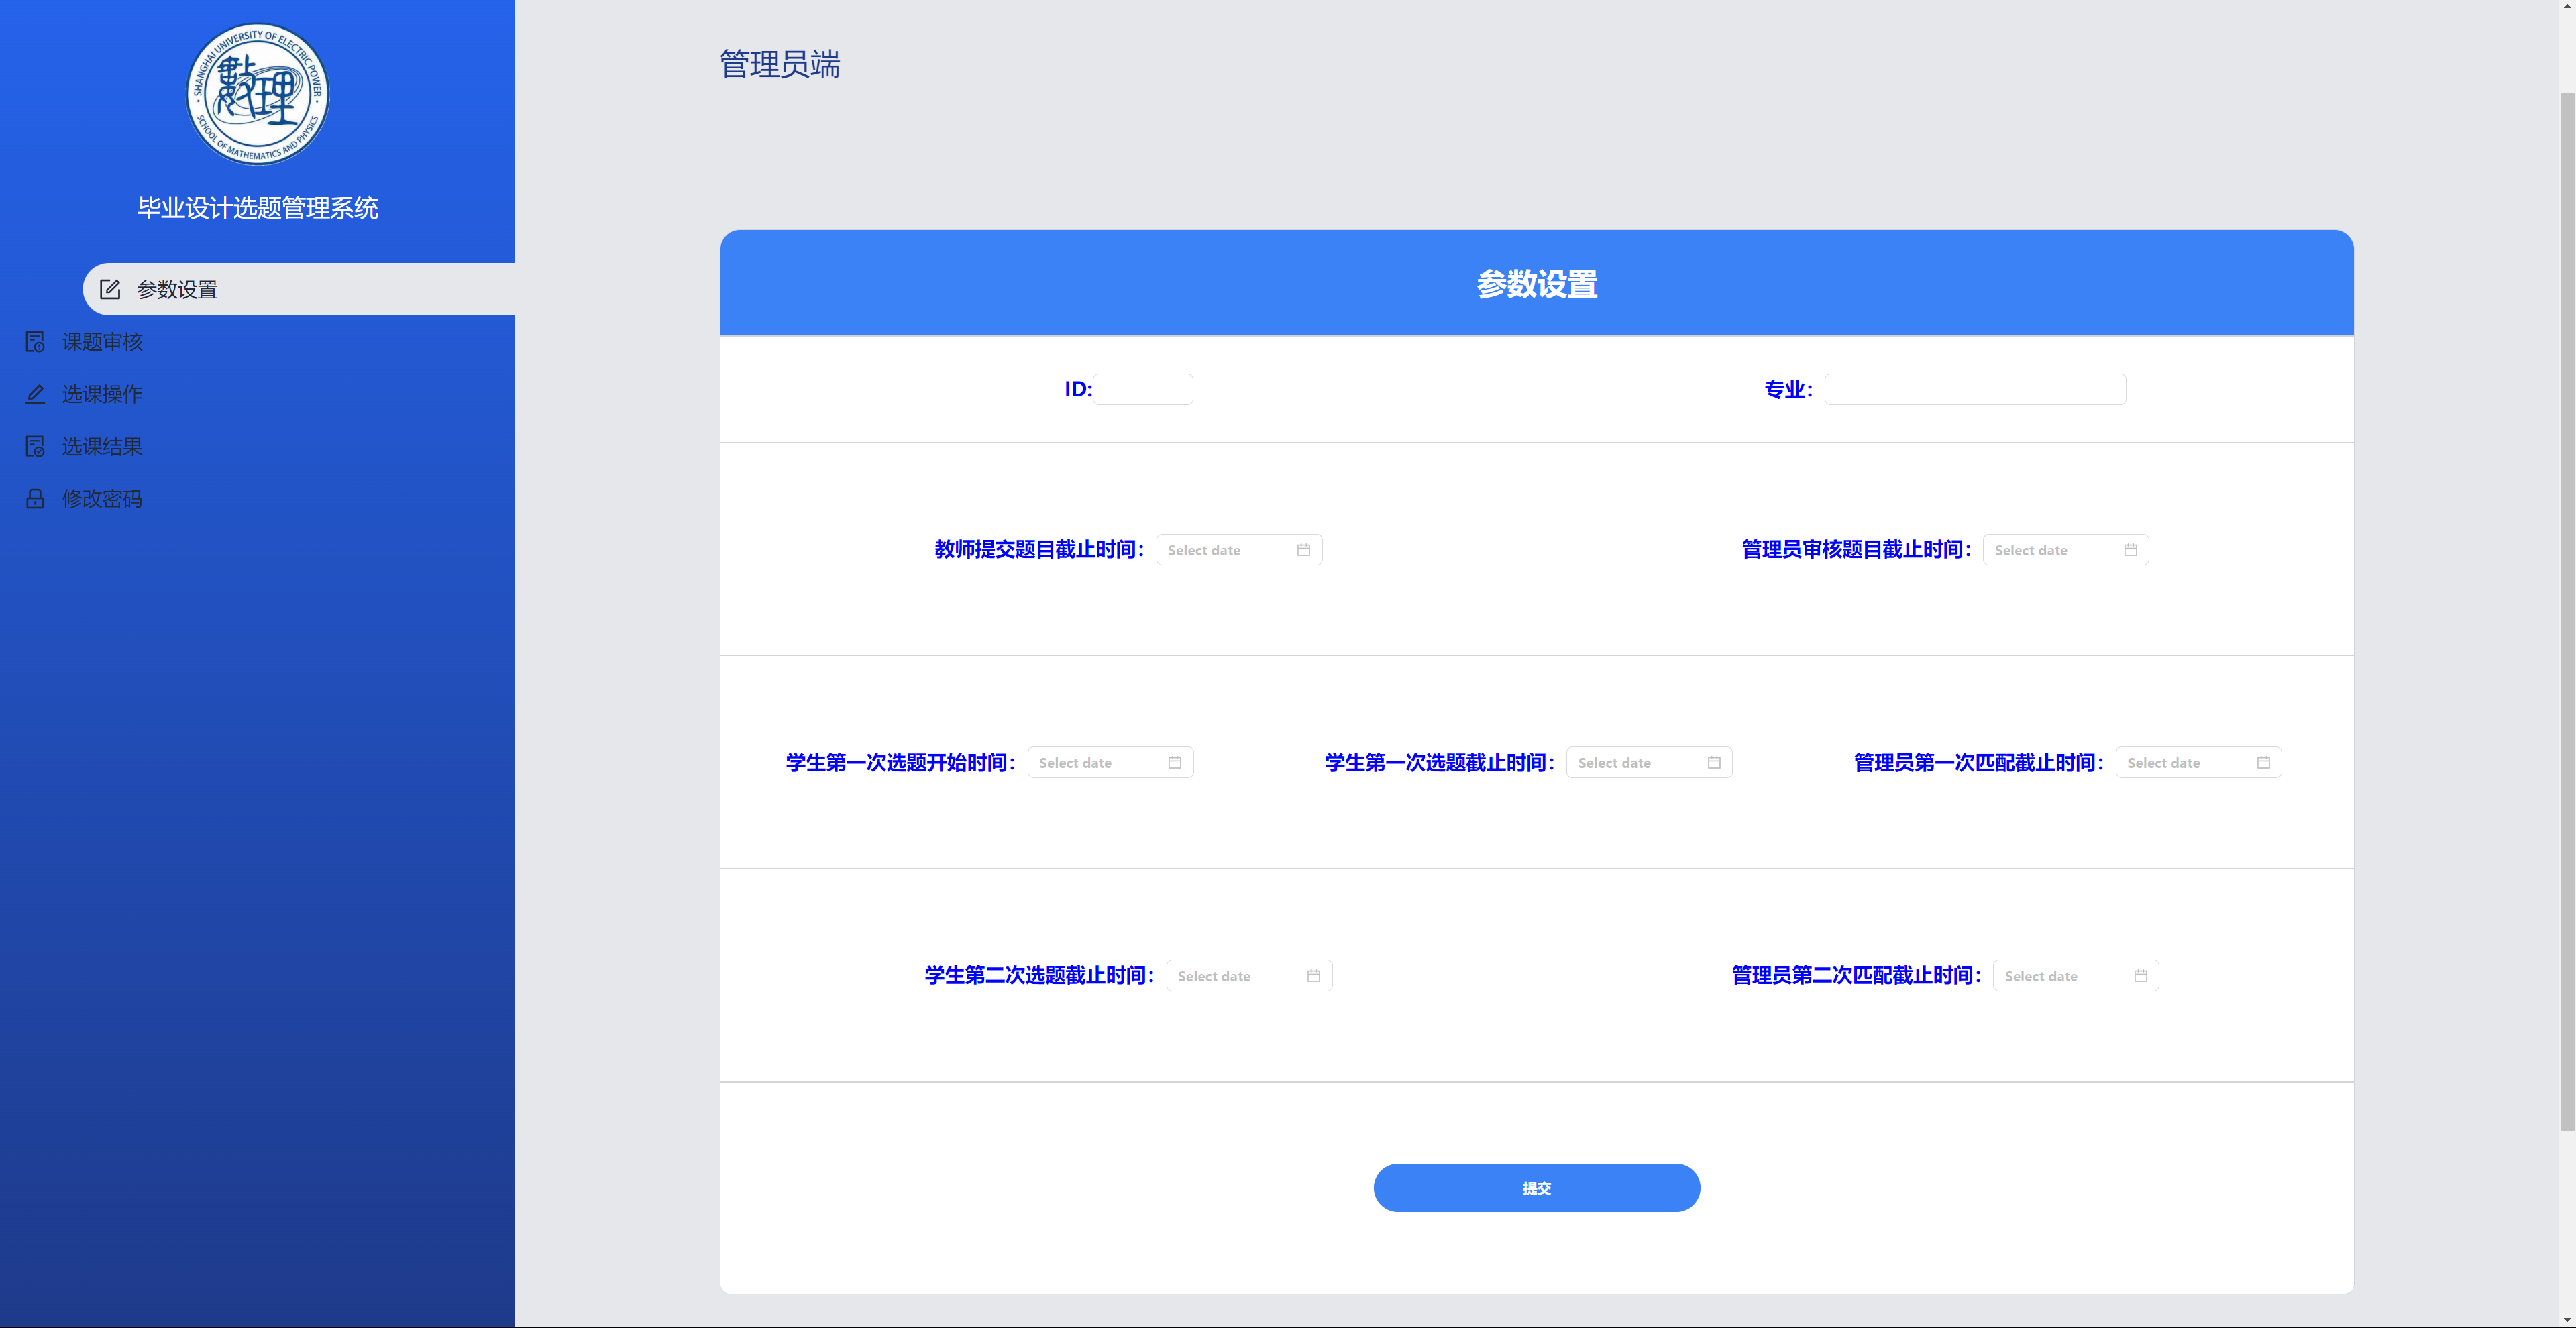
\includegraphics[width=1\textwidth]{管理员端01.png} % 插入图片并指定宽度
    \caption{管理员端-参数设置} % 添加图片标题
    \label{fig:manager01} % 为图片添加标签,以便在文本中引用
\end{figure}

\clearpage

\subsubsection{课题审核:}
在课题审核模块中,系统管理员可以查看到课题的编号、名称、指导老师、所属专业年级以及审核情况,
并对课题进行审核操作。
\begin{figure}[h]
    \centering
    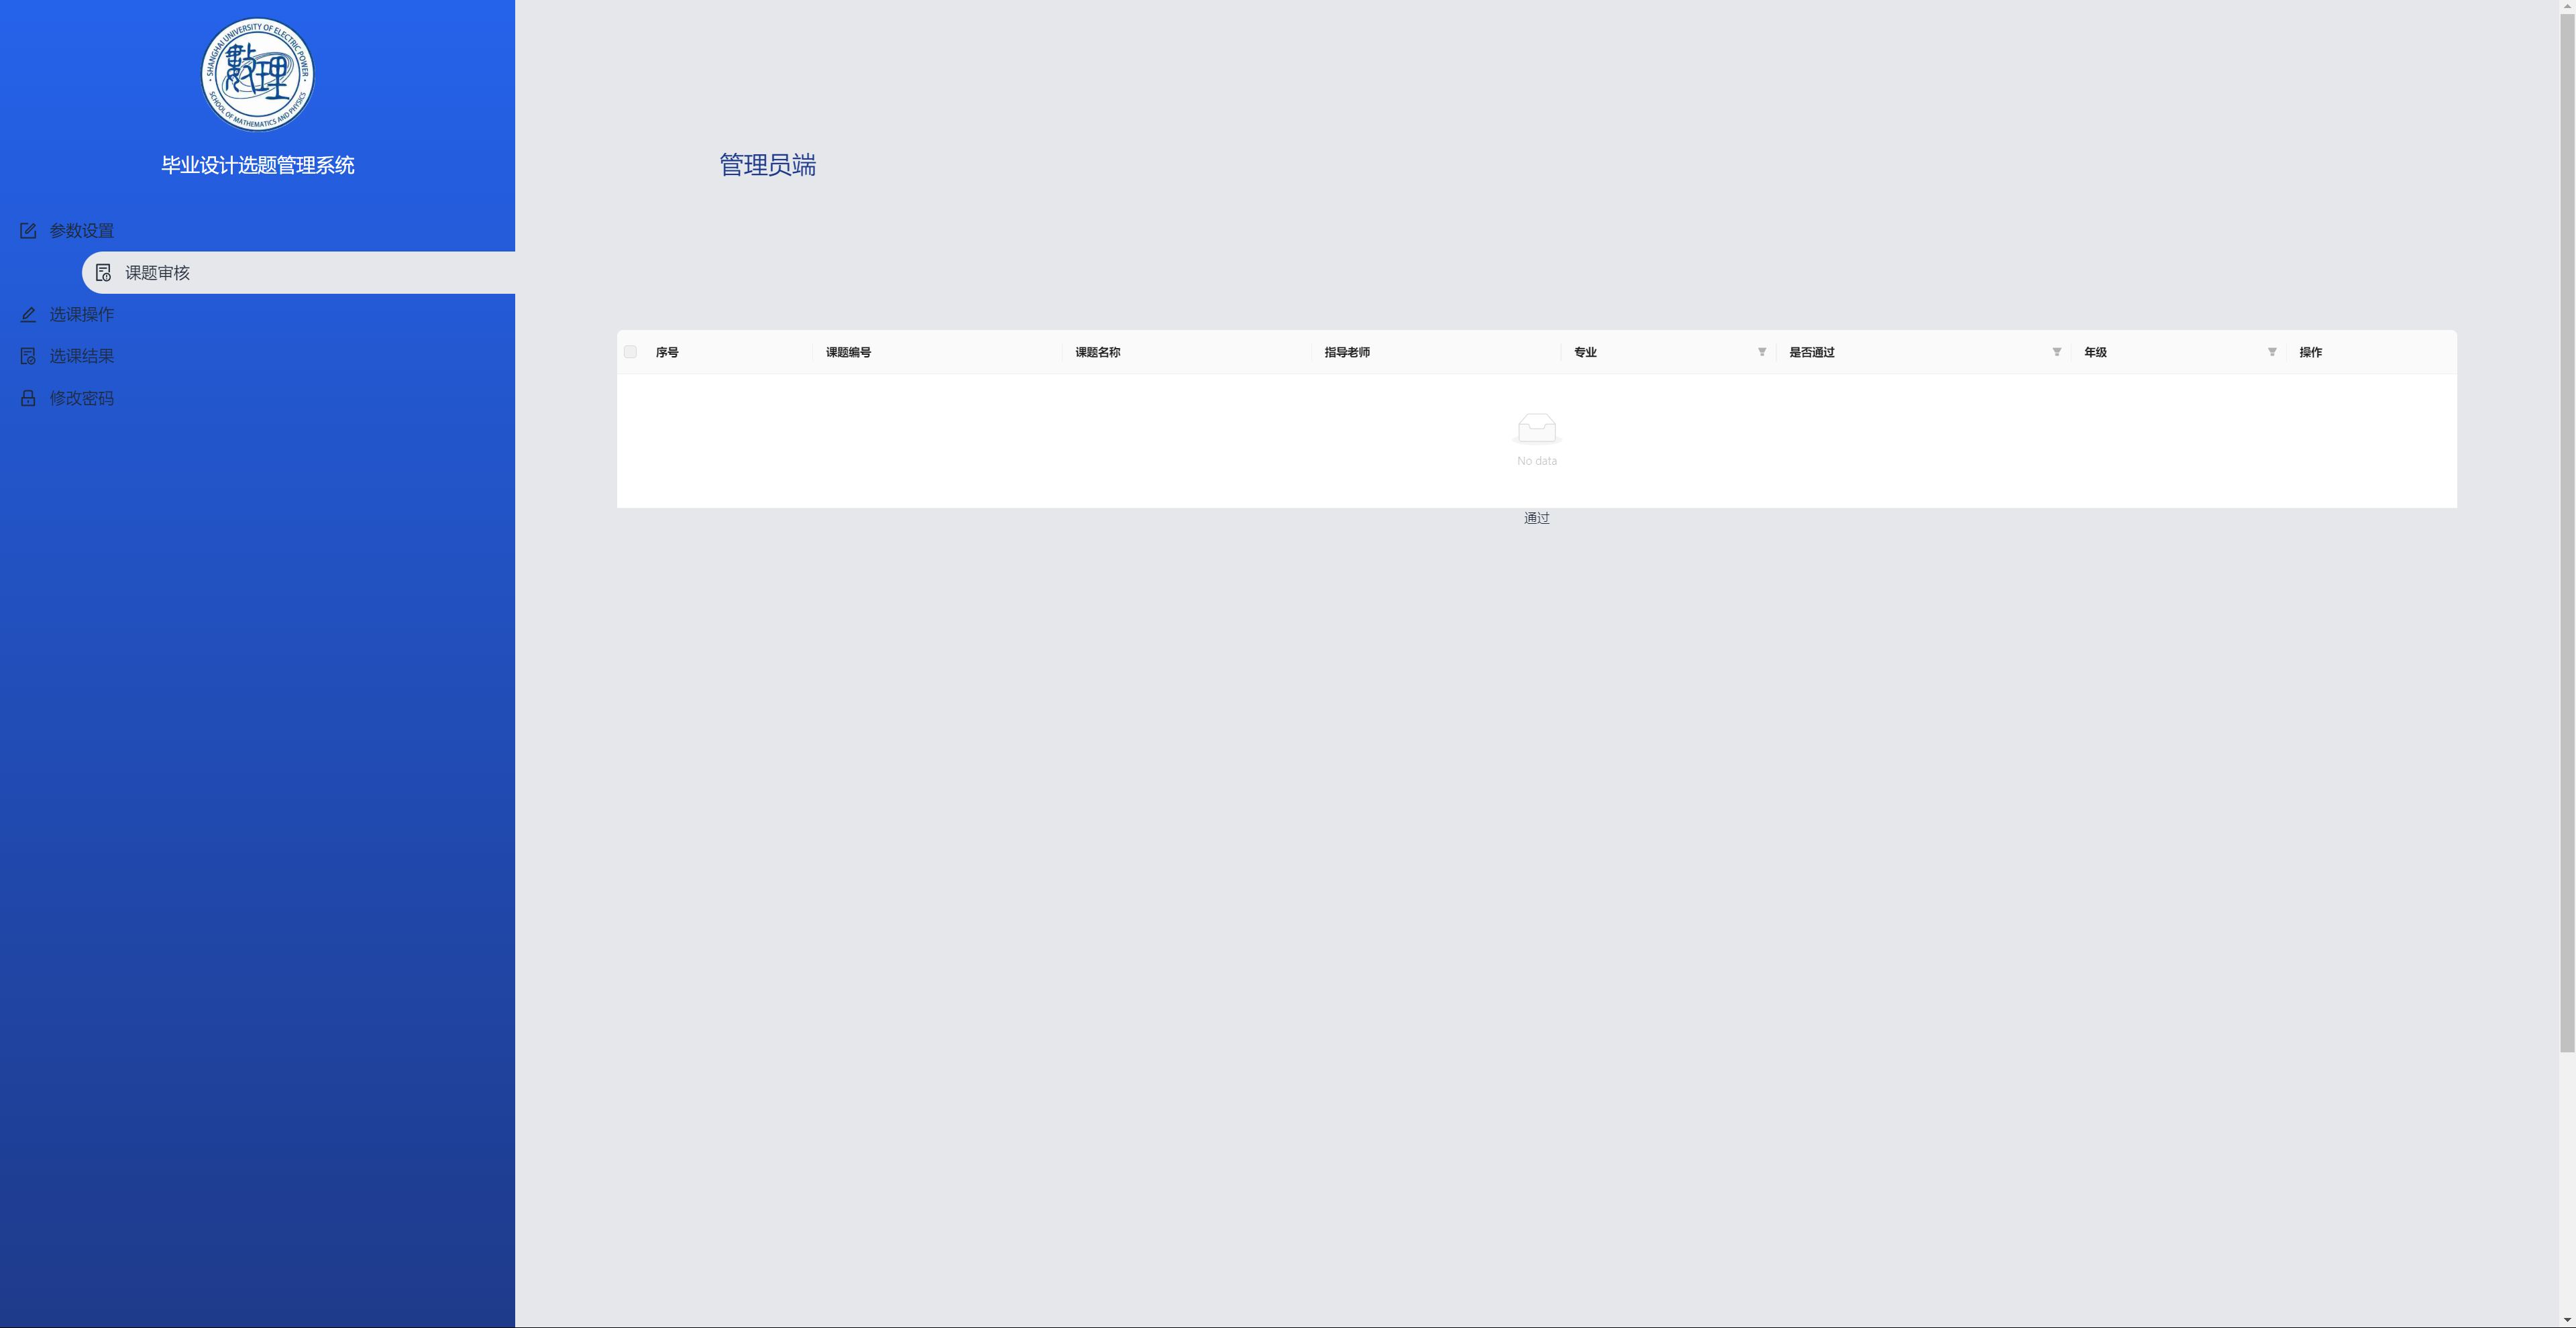
\includegraphics[width=1\textwidth]{images/管理员端02.png}
    \caption{管理员端-课题审核}
    \label{fig:manager02}
\end{figure}

\subsubsection{选课操作:}
在选课操作界面,系统管理员可以设置提前批选课的学号以及课号,
查看第一第二次选题分配情况,并且提供了导出选题匹配结果以及选题失败同学名单的选项。
\begin{figure}[h]
    \centering
    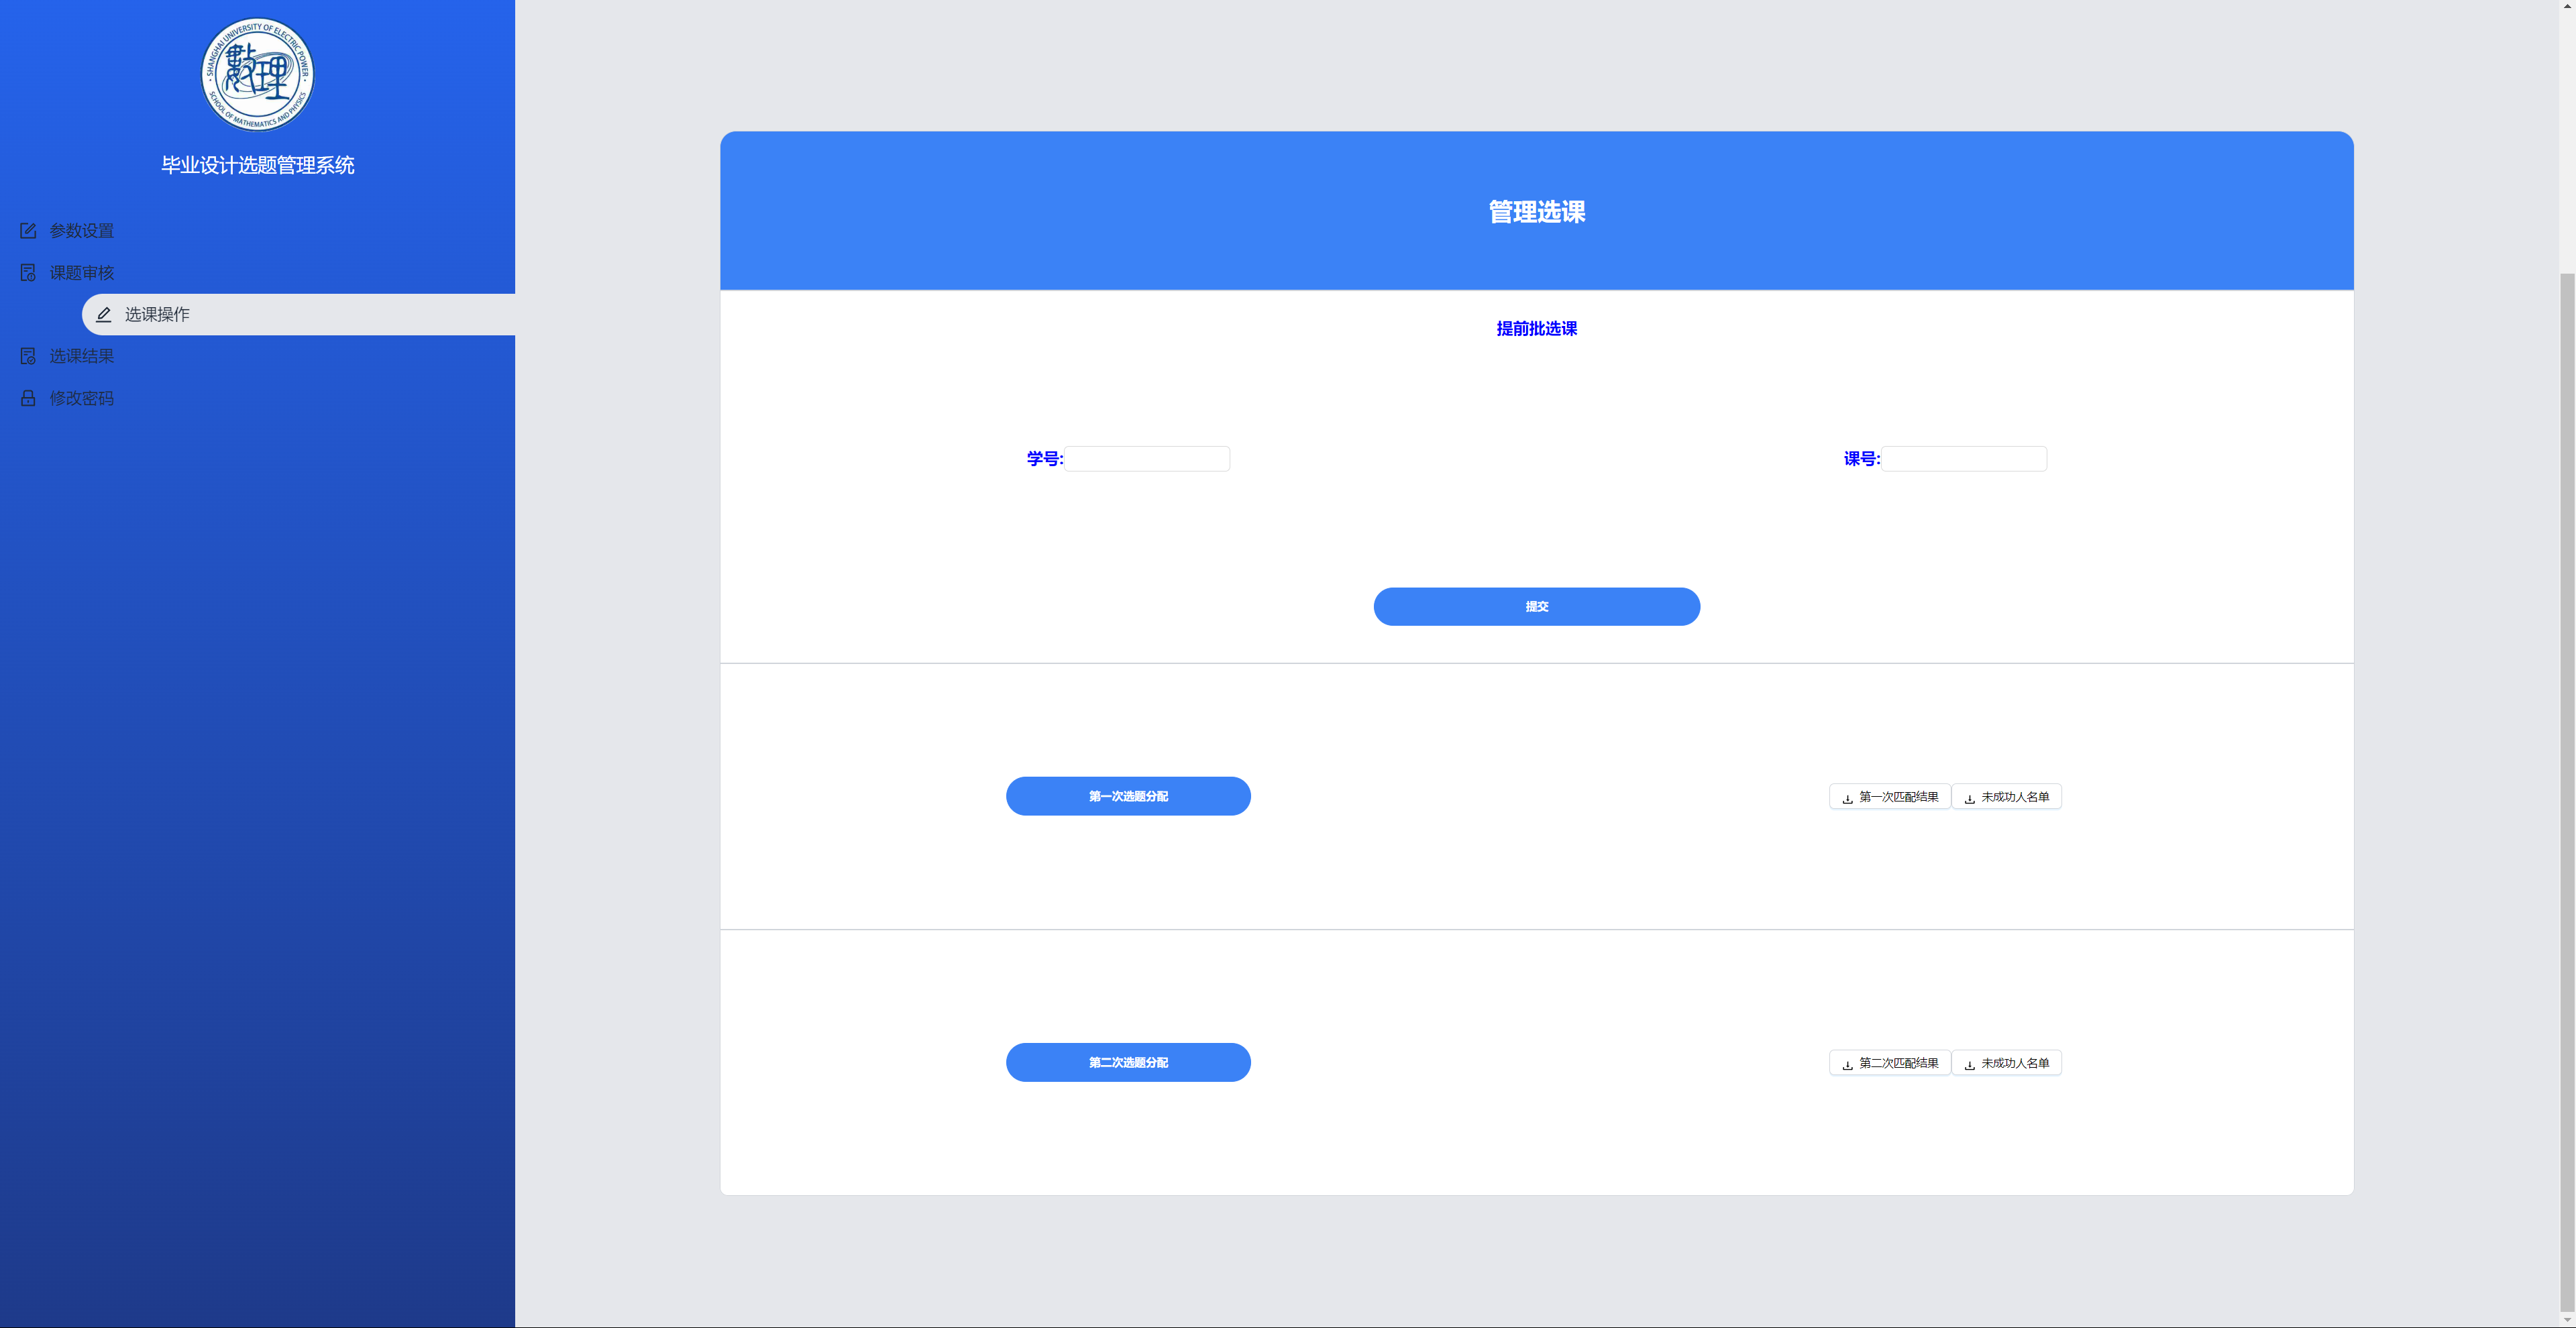
\includegraphics[width=1\textwidth]{管理员端03.png}
    \caption{管理员端-选课操作}
    \label{fig:manager03}
\end{figure}

\subsubsection{选题结果:}
在选题结果模块中,管理员可以查看学生选课的课题编号、学号、姓名、课题名称、指导老师以及学年的信息,
并且增加了按年份筛选、搜索课题和导出选课结果表格的功能;
\begin{figure}[h]
    \centering
    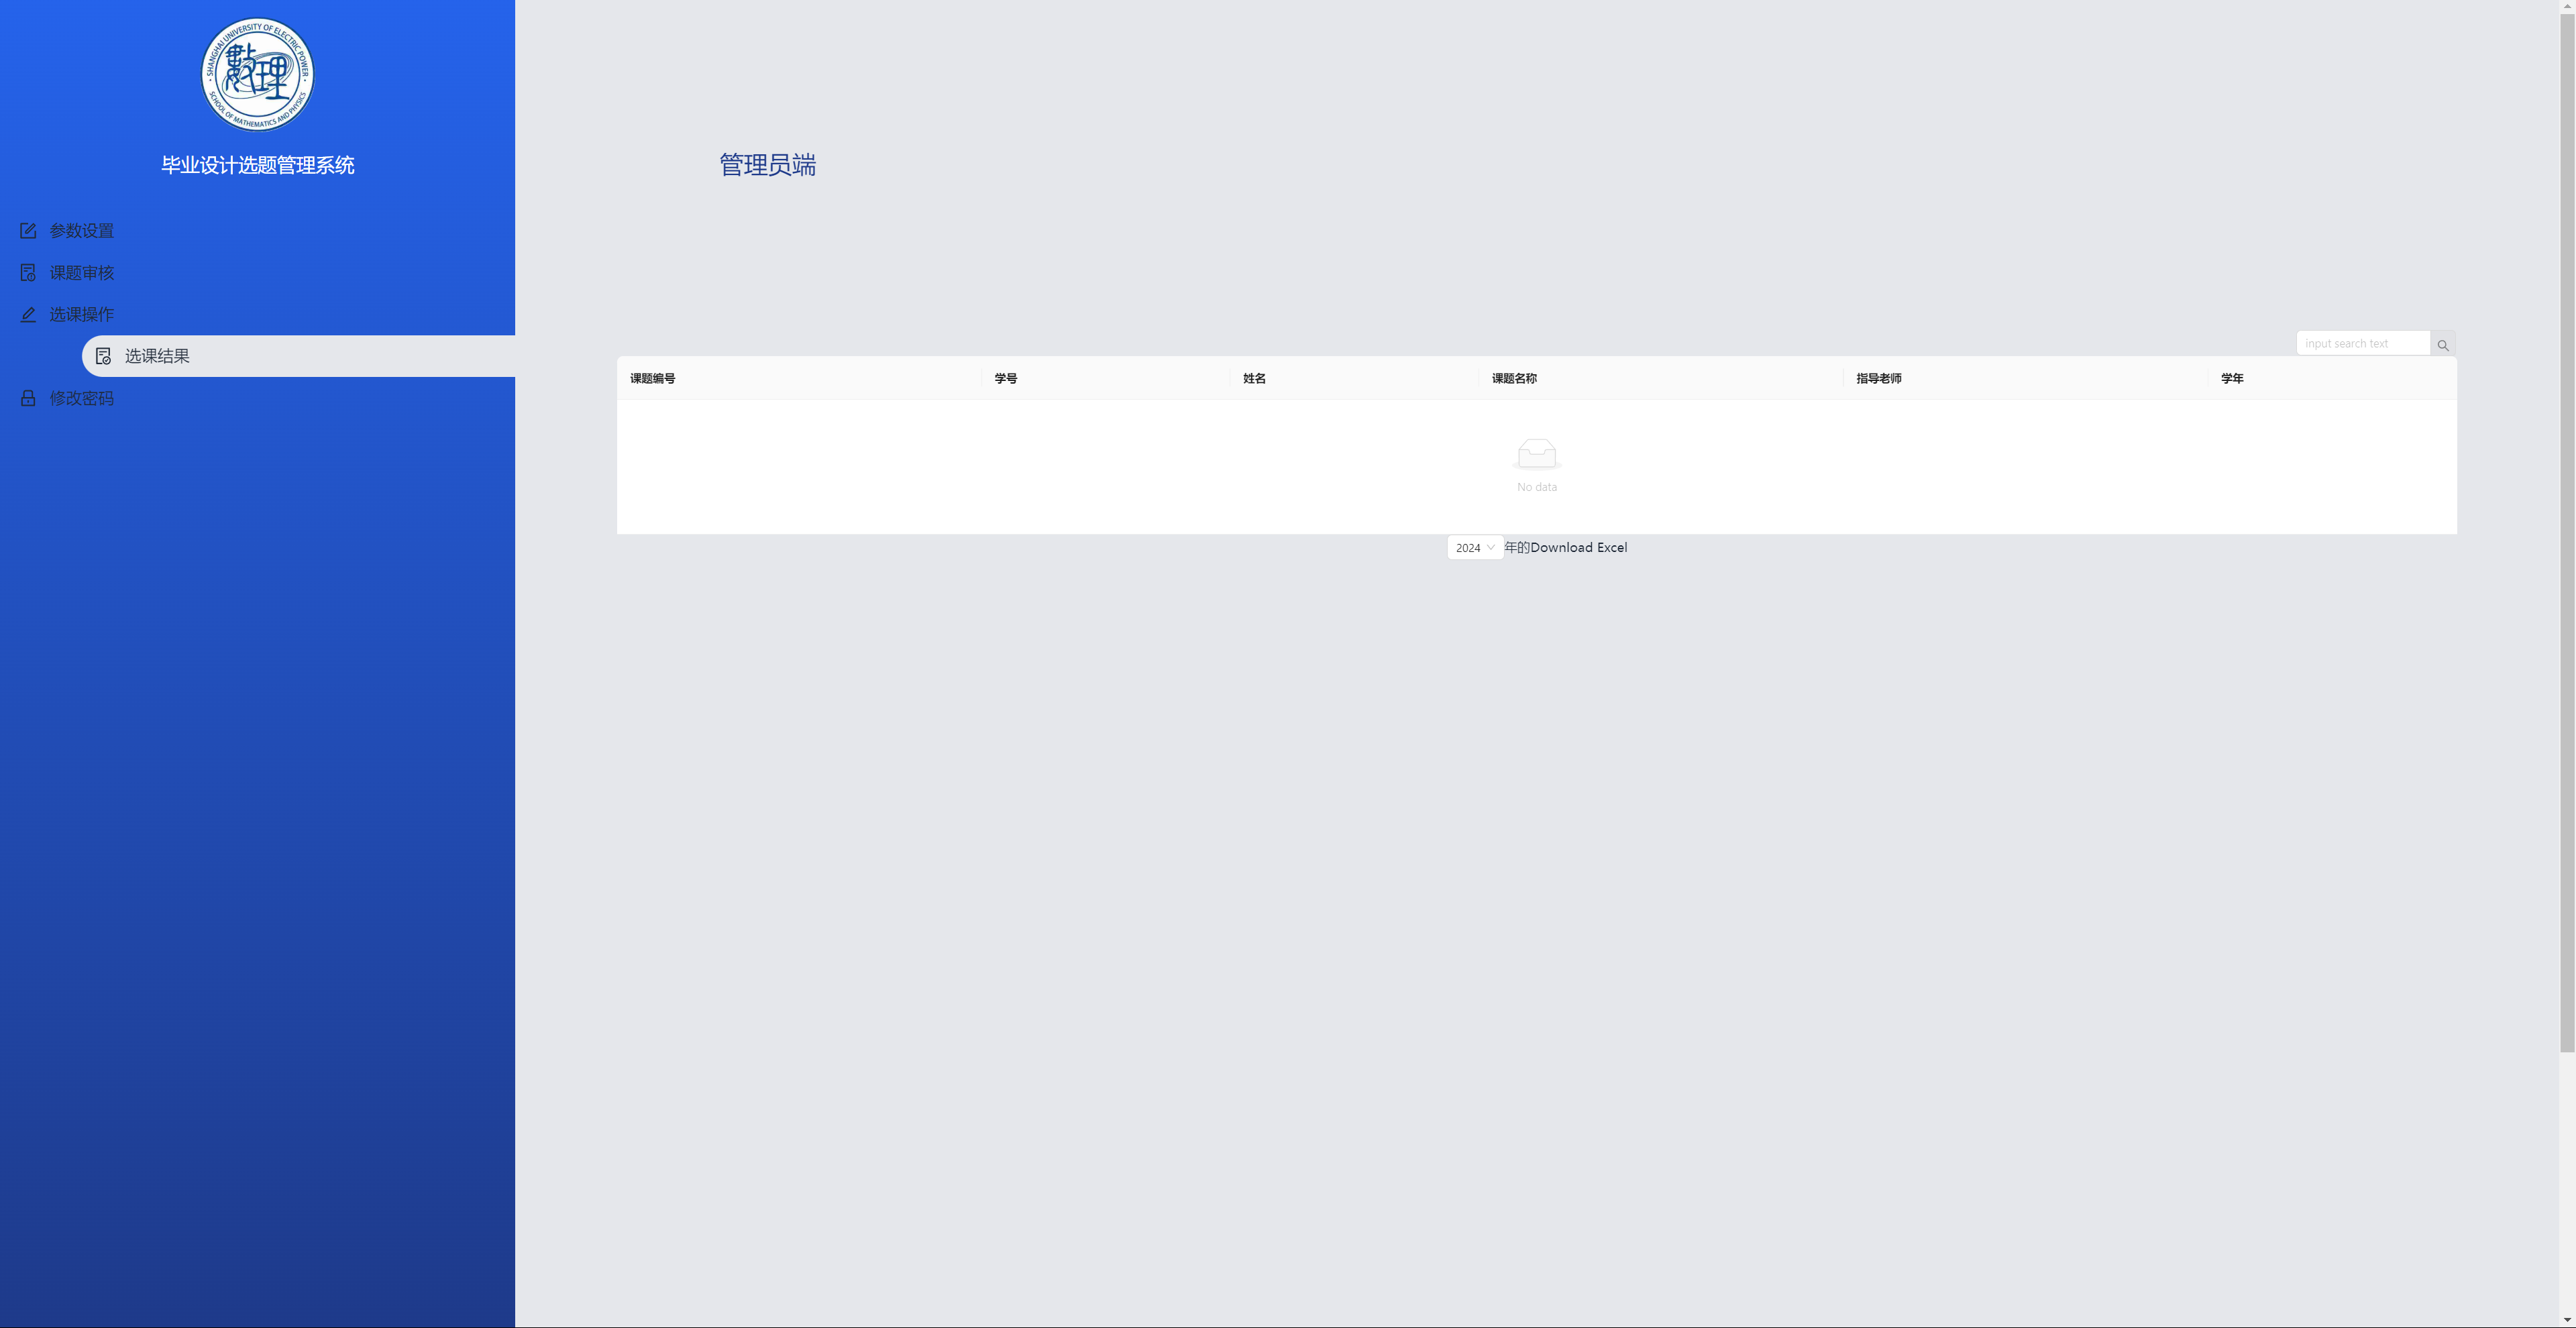
\includegraphics[width=1\textwidth]{管理员端04.png}
    \caption{管理员端-选题结果}
    \label{fig:manager04}
\end{figure}

\subsubsection{修改密码:}
最后,考虑到师生会出现忘记密码的普遍情况,
增加了修改密码这一模块用于重置教师和学生的密码。
\begin{figure}[ht]
    \centering
    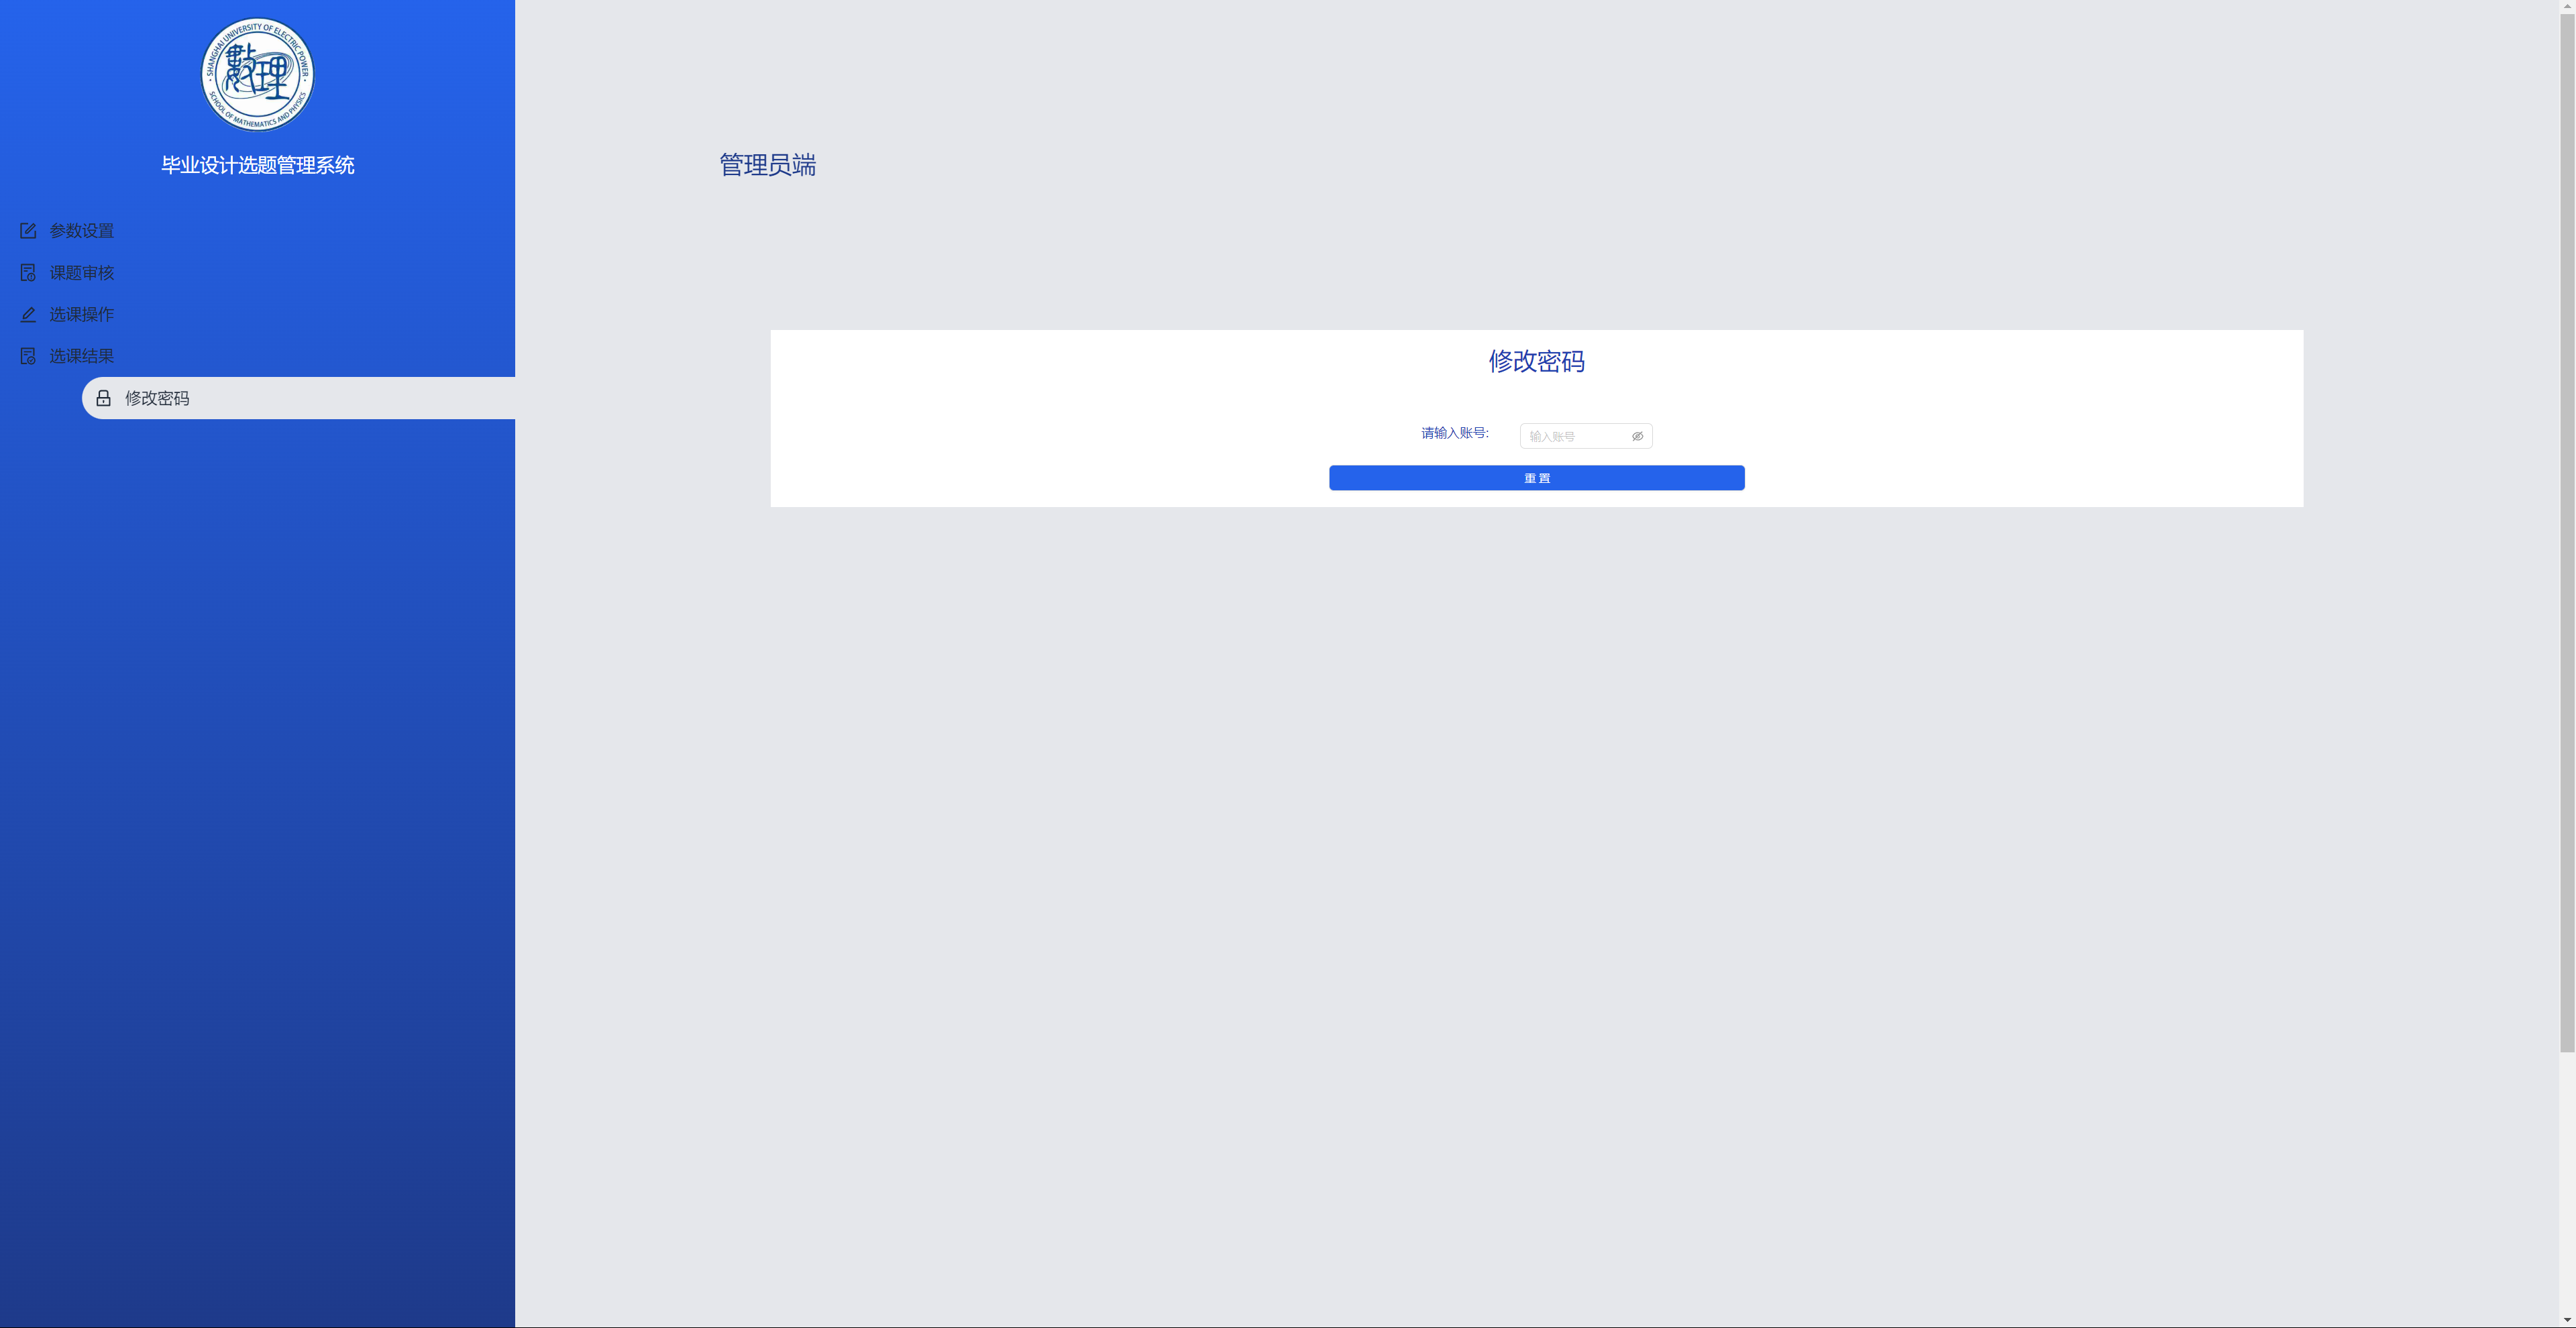
\includegraphics[width=1\textwidth]{管理员端05.png}
    \caption{管理员端-修改密码}
    \label{fig:manager05}
\end{figure}


\subsection{教师端}
\subsubsection{课题提交:}
提供教师输入课题的各项具体信息。
\begin{figure}[ht]
    \centering
    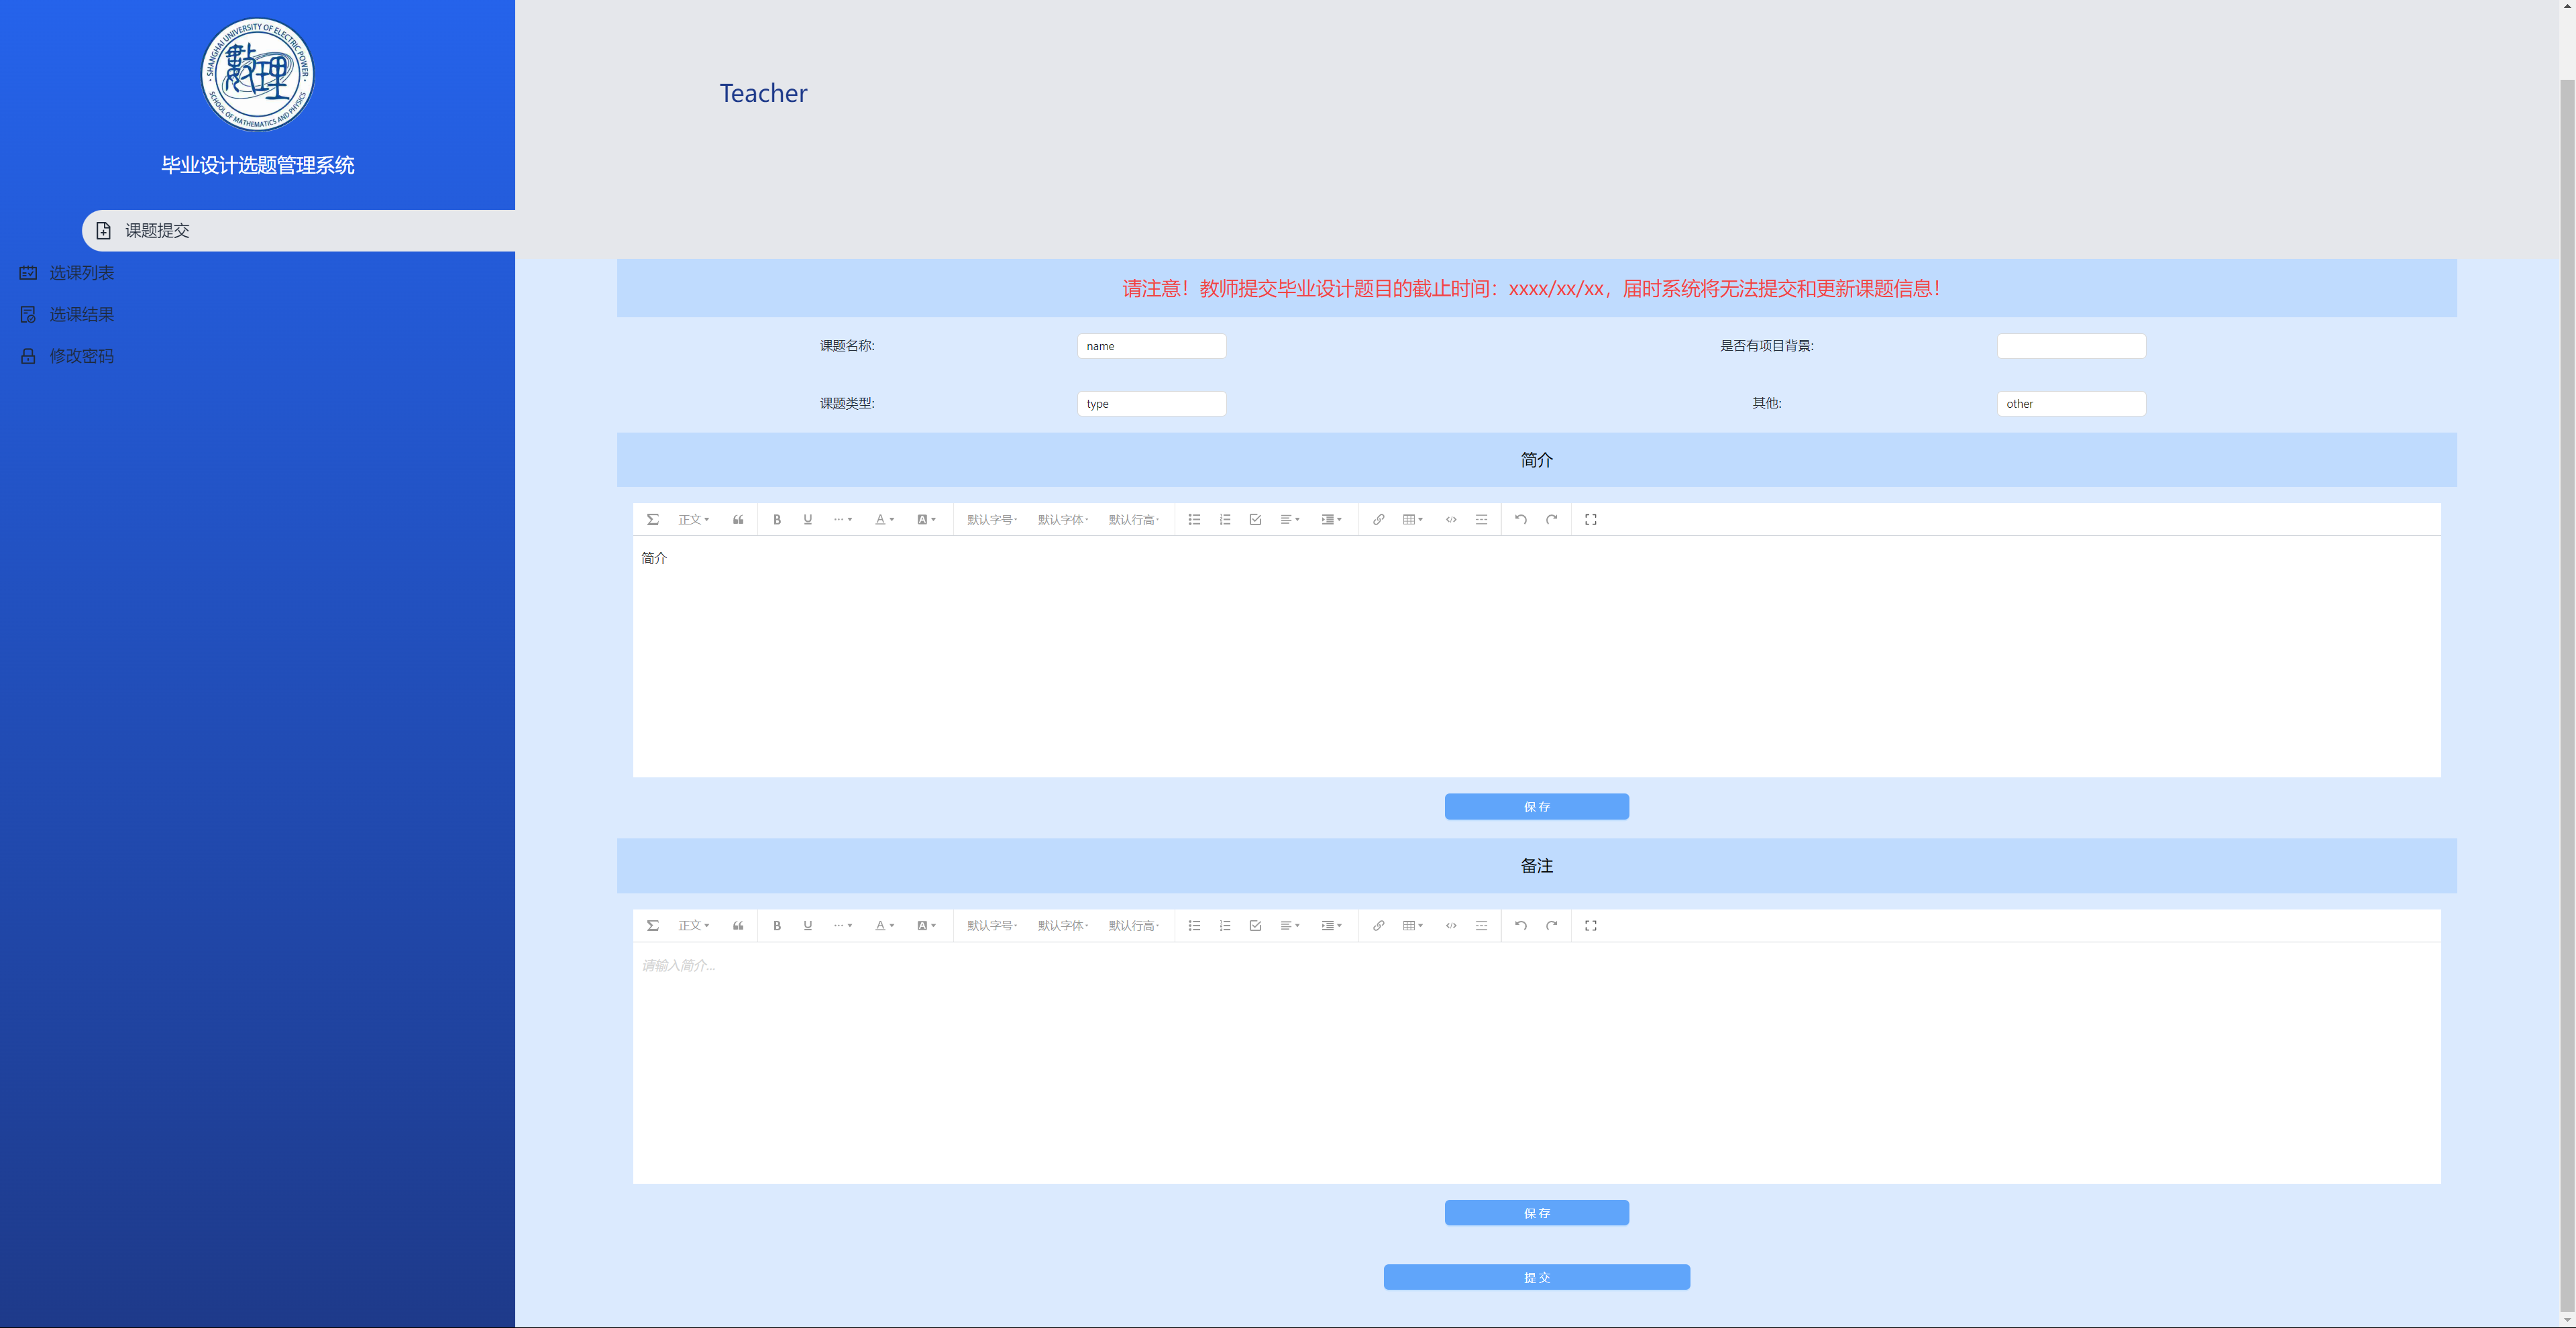
\includegraphics[width=1\textwidth]{教师端01.png}
    \caption{管理员端-课题提交}
    \label{fig:teacher01}
\end{figure}

\subsubsection{选课列表:}
查看提交的课题的信息并进行修改删除等操作。
\begin{figure}[ht]
    \centering
    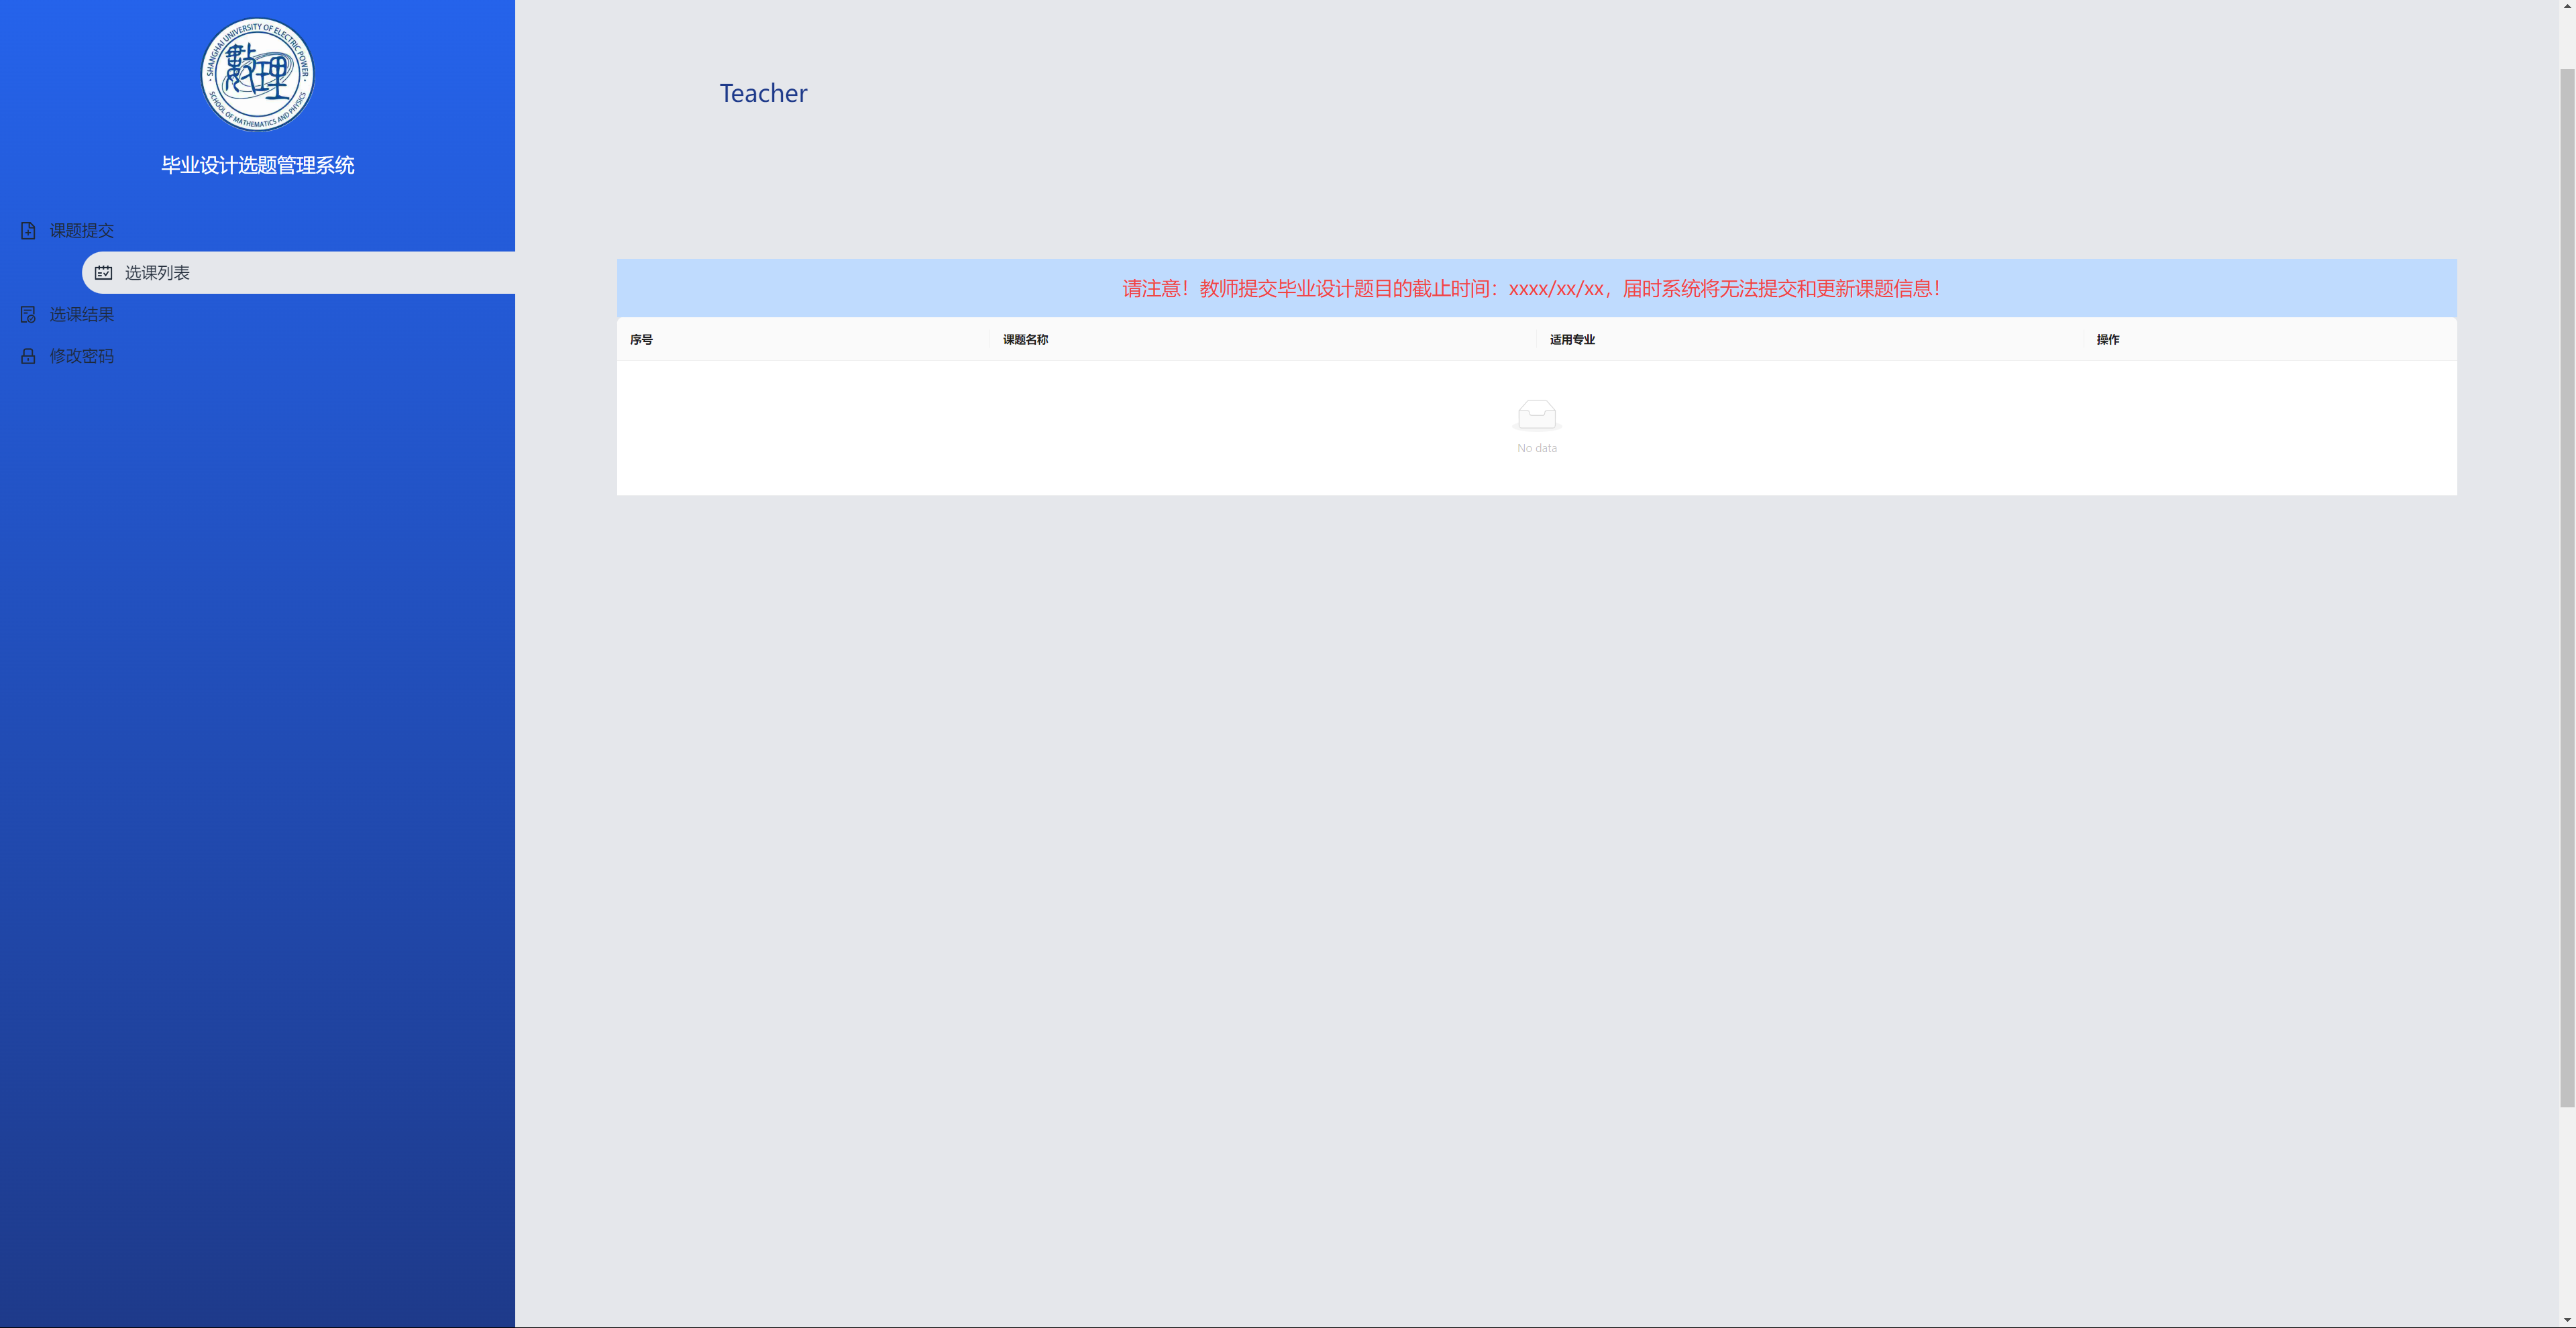
\includegraphics[width=1\textwidth]{教师端02.png}
    \caption{教师端-选课列表}
    \label{fig:teacher02}
\end{figure}

\subsubsection{选课结果:}
查看学生的选题结果信息,
包括学生姓名学号专业班级联系方式,
便于老师了解自己课题的选题情况。
\begin{figure}[ht]
    \centering
    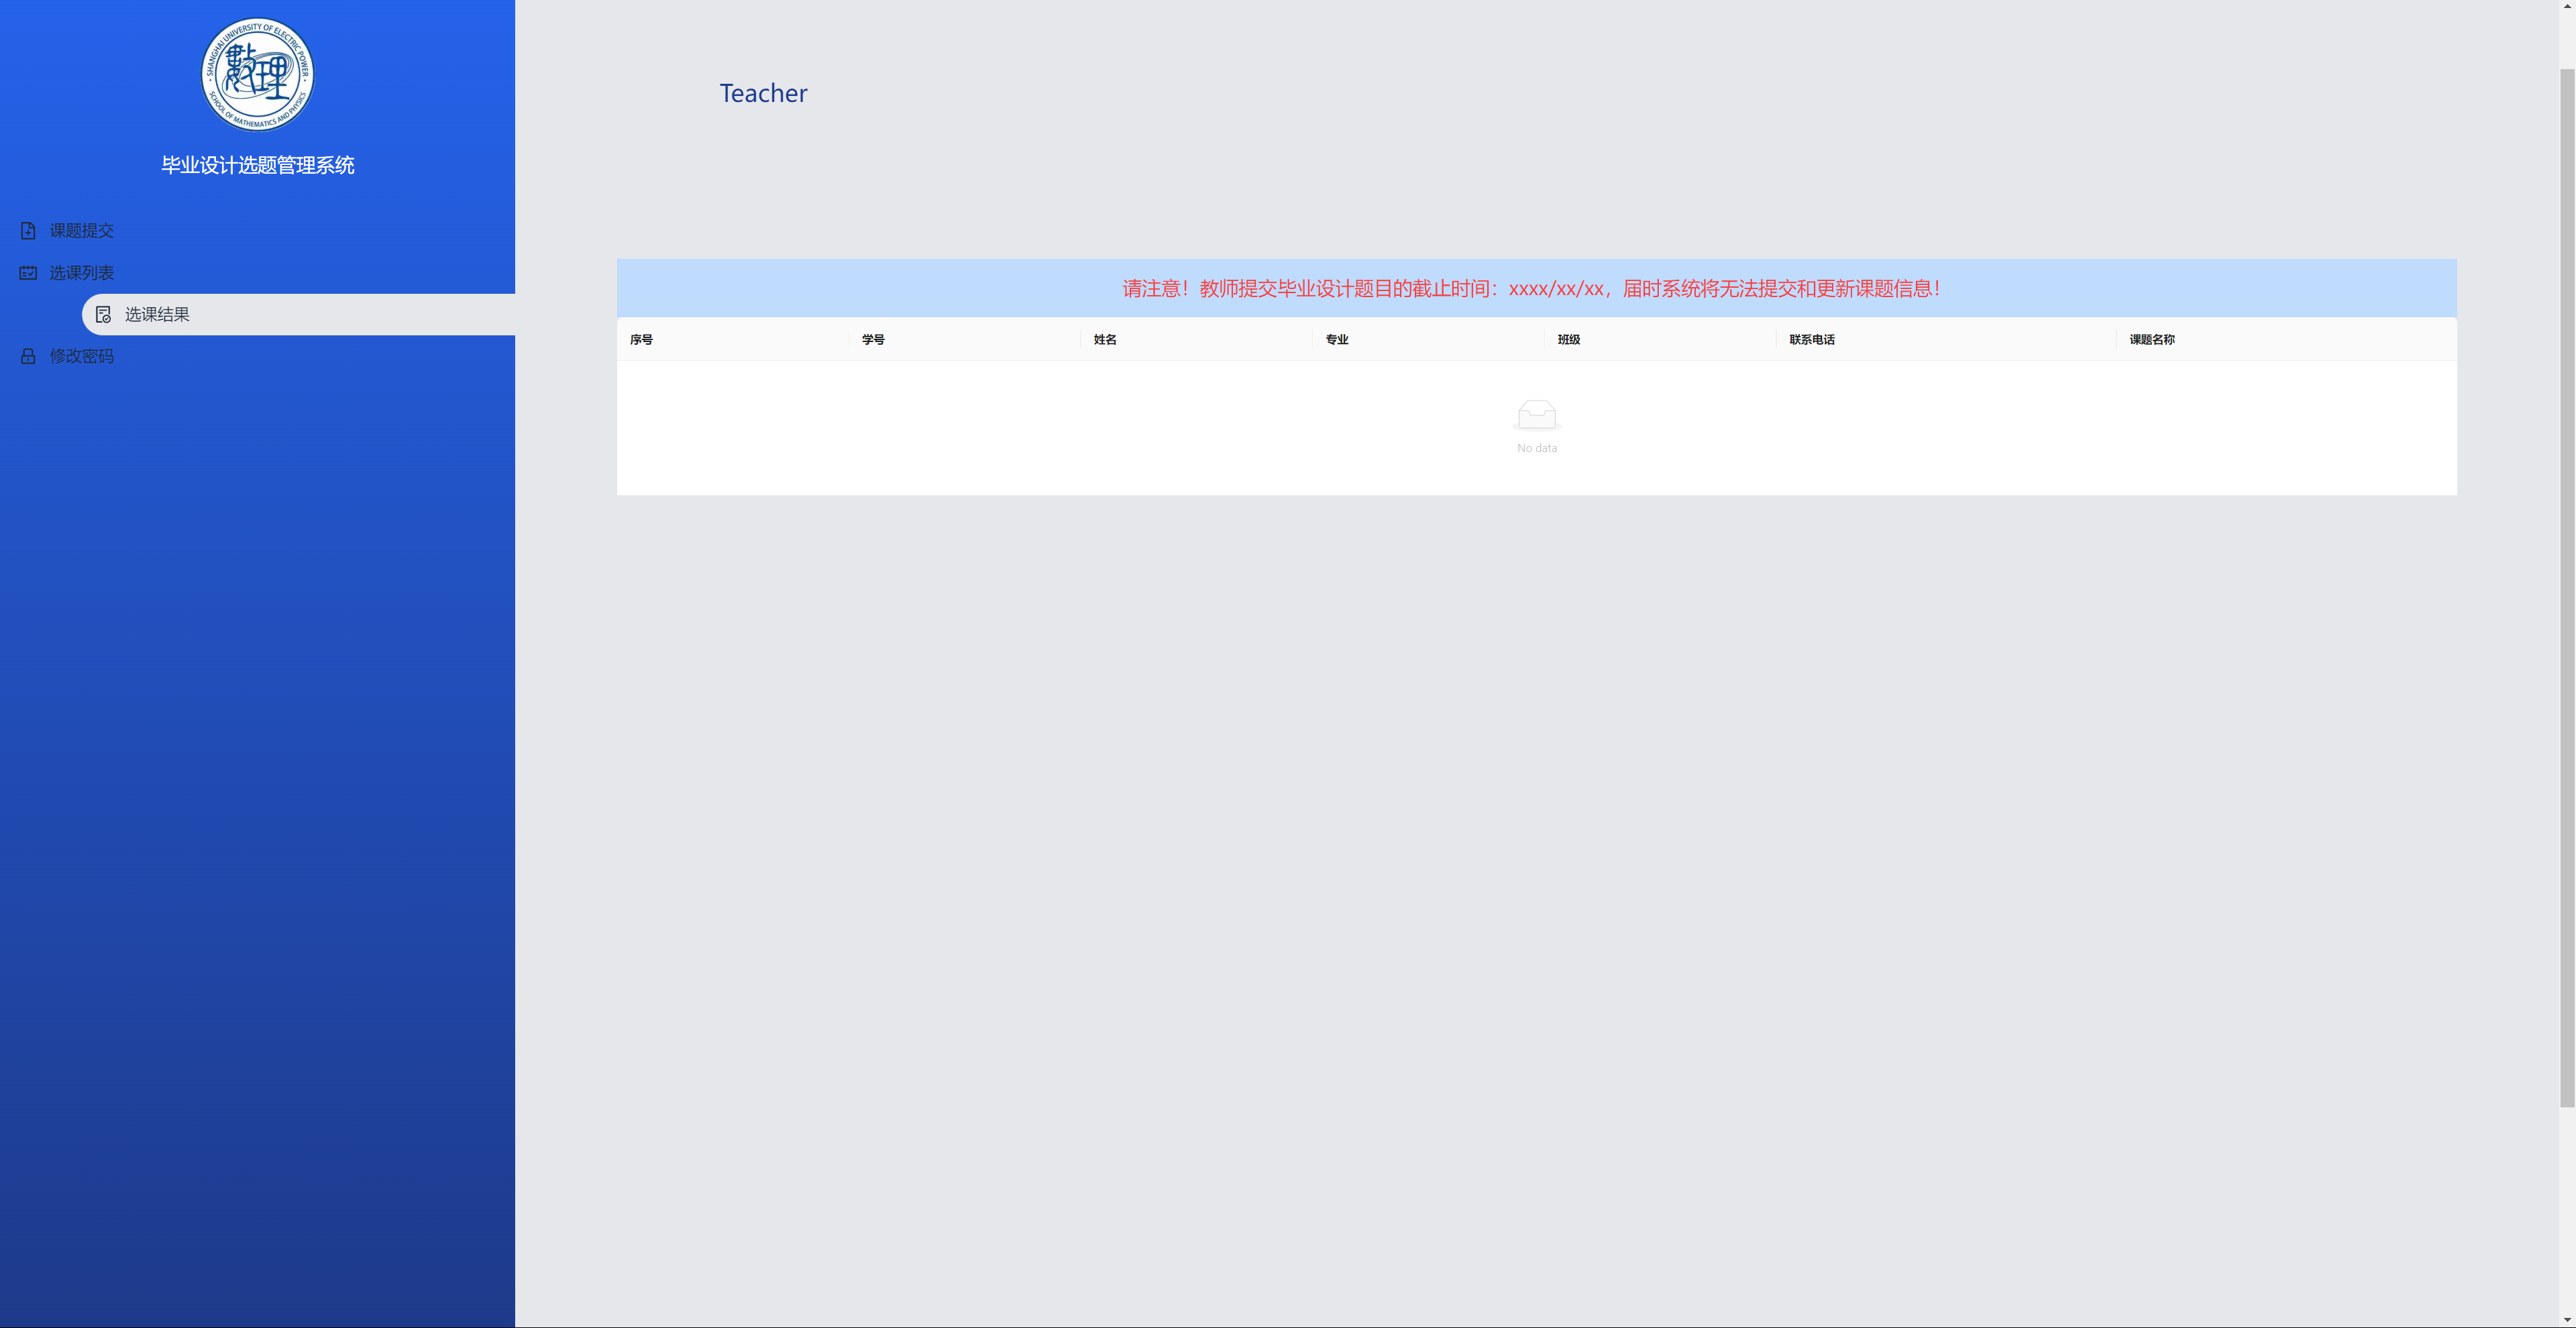
\includegraphics[width=1\textwidth]{教师端03.png}
    \caption{教师端-选课结果}
    \label{fig:teacher03}
\end{figure}

\subsubsection{修改密码:}
提供了教师更新密码的窗口。
\begin{figure}[ht]
    \centering
    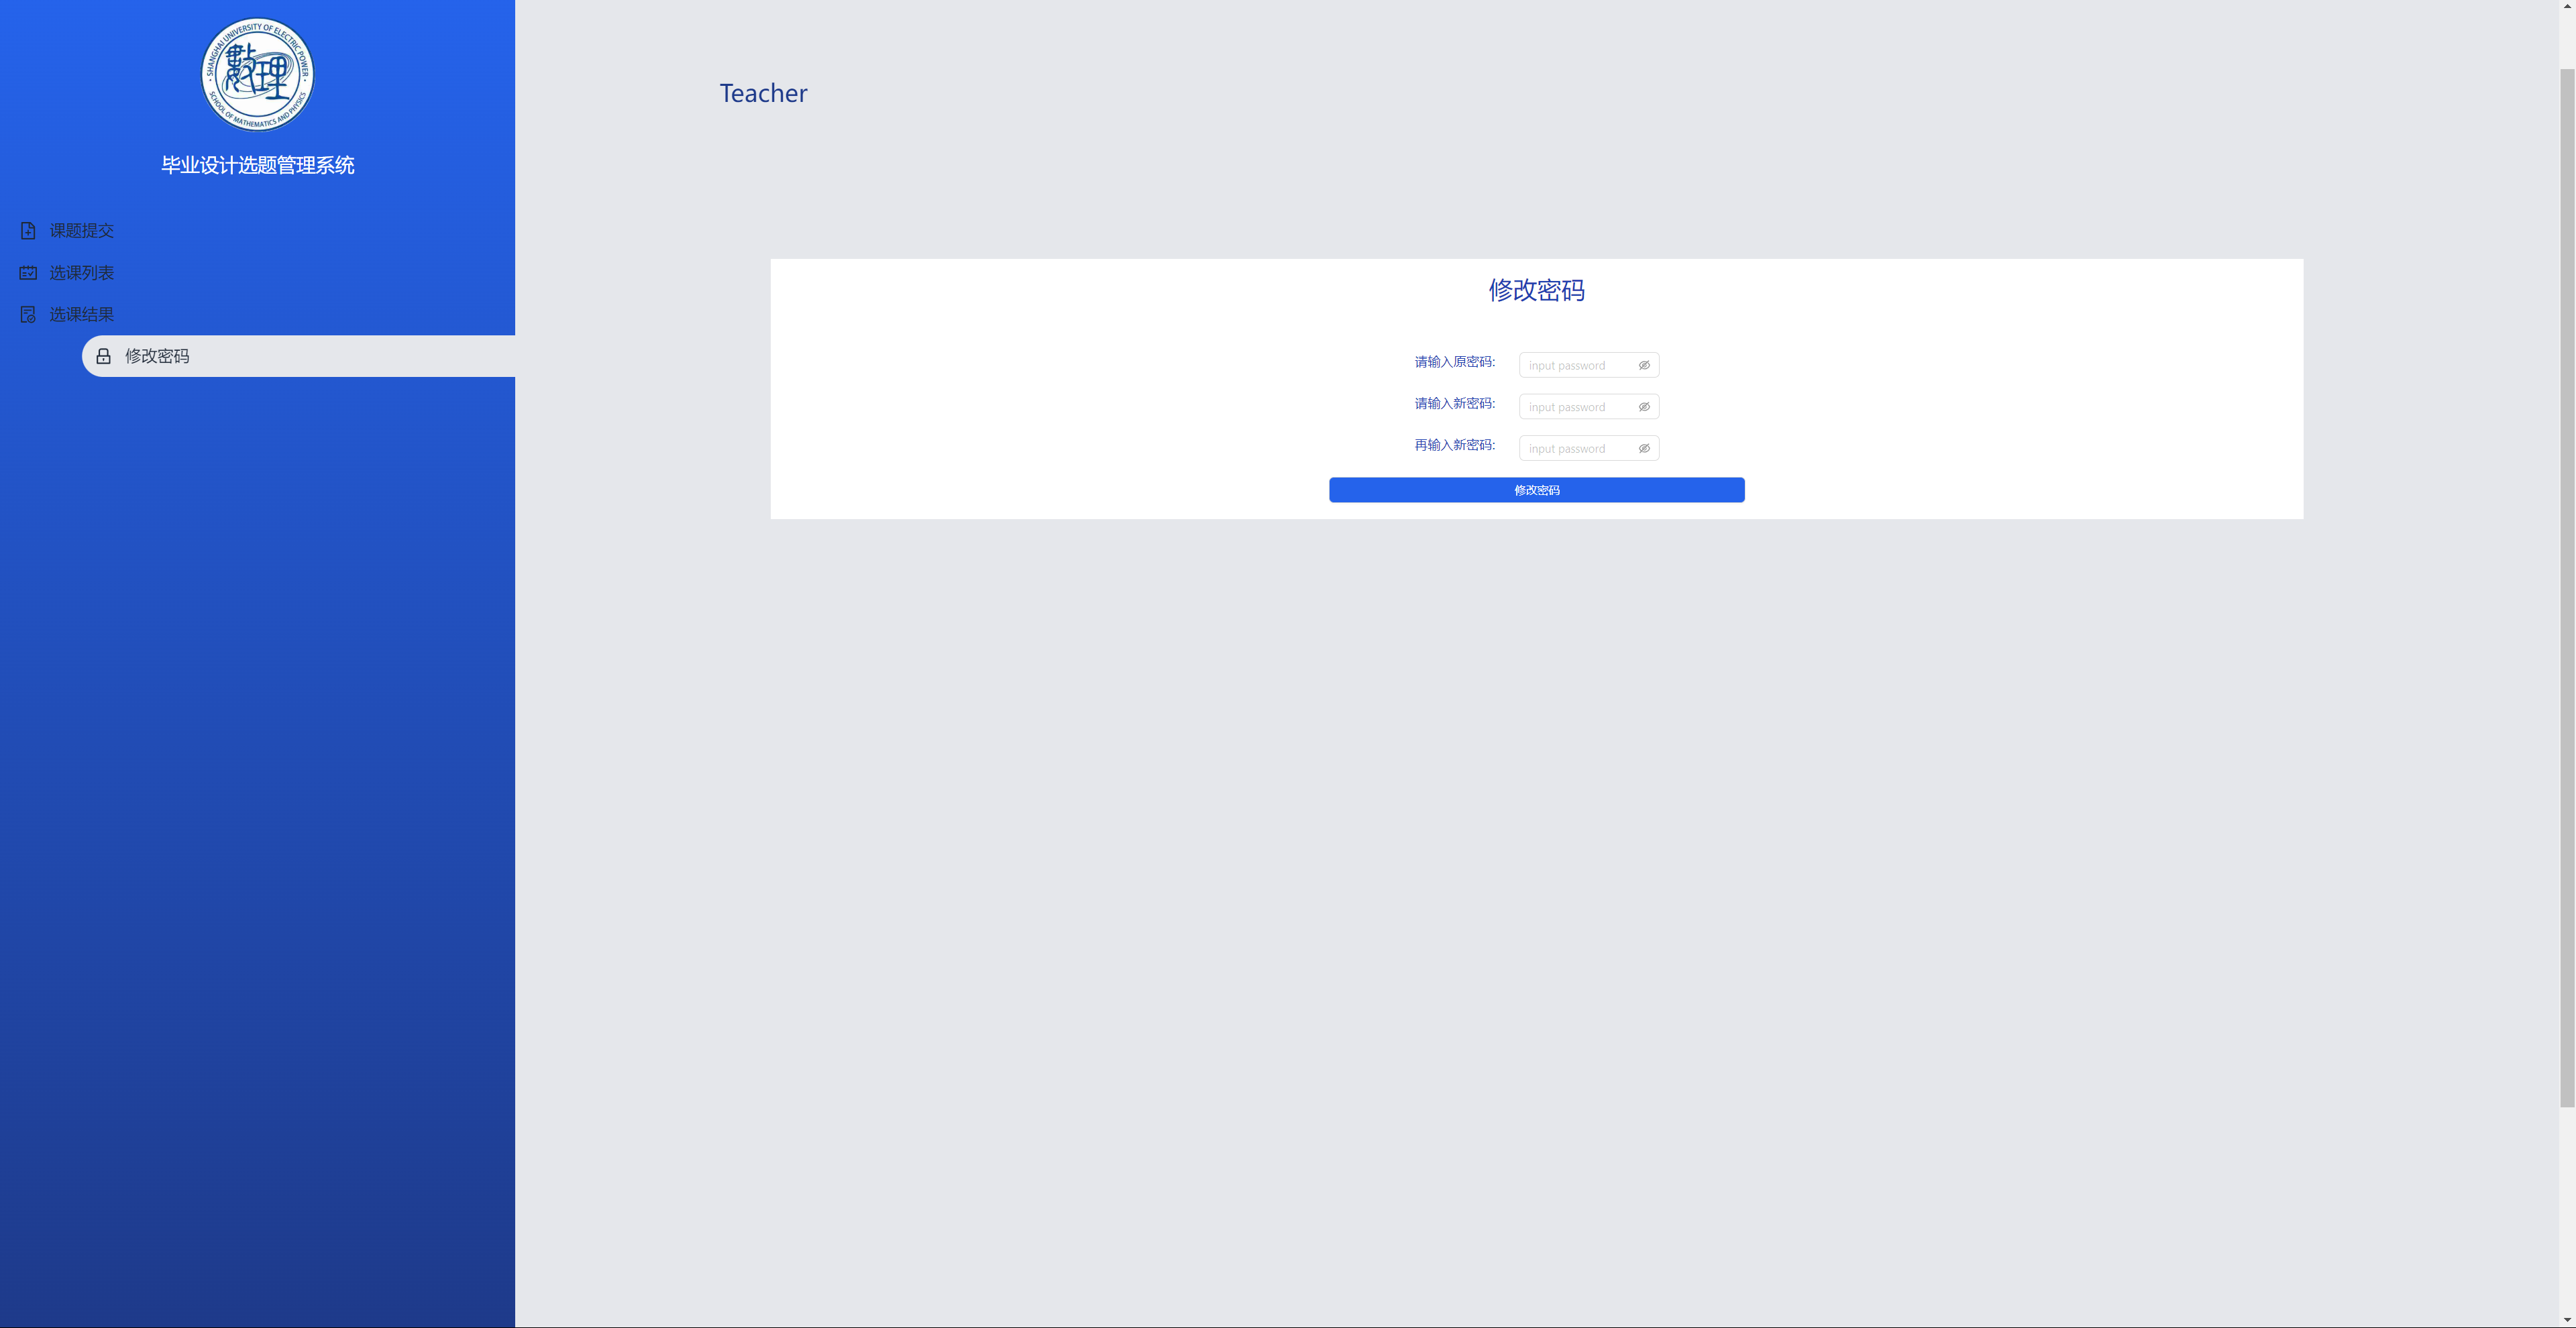
\includegraphics[width=1\textwidth]{教师端04.png}
    \caption{教师端-修改密码}
    \label{fig:teacher04}
\end{figure}


\subsection{普通用户端}
\subsubsection{选题规则:}
在这里学生可以查看数理学院毕业论文(设计)选题规则。
\begin{figure}[h]
    \centering
    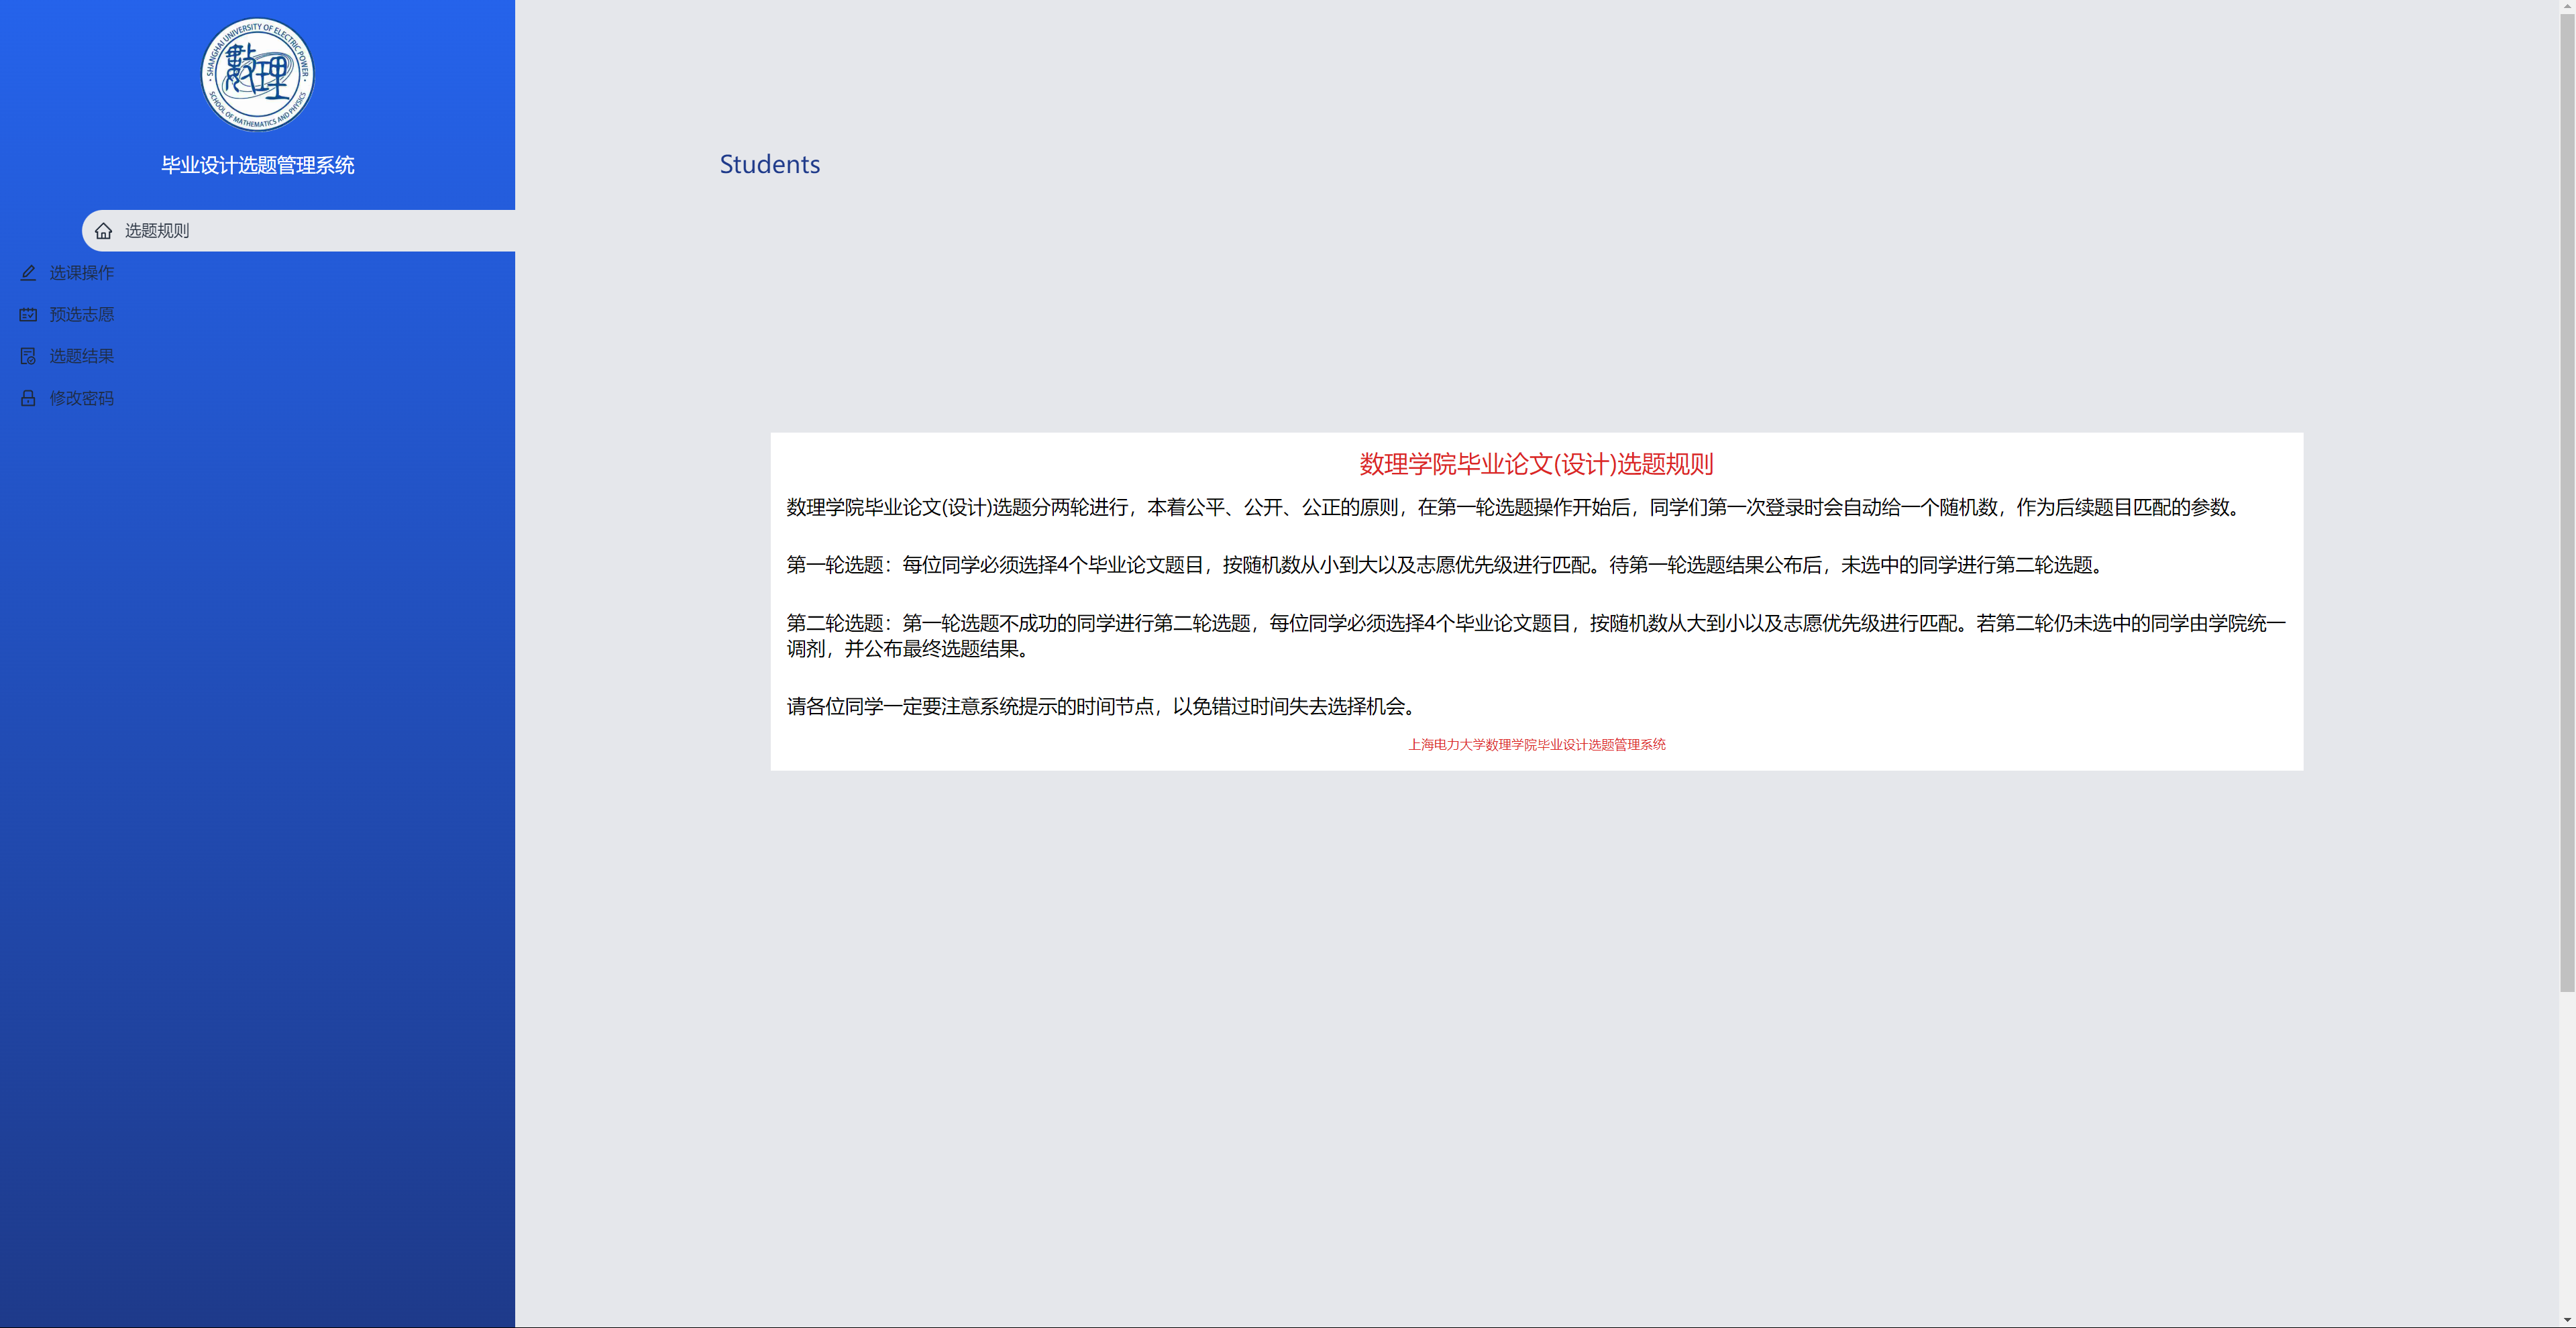
\includegraphics[width=1\textwidth]{学生端01.png}
    \caption{学生端-选题规则}
    \label{fig:student01}
\end{figure}

\subsubsection{选课操作:}
在学生端的选课操作模块中,学生可以查看课题的编号、名称以及类别进行选题操作。
\begin{figure}[h]
    \centering
    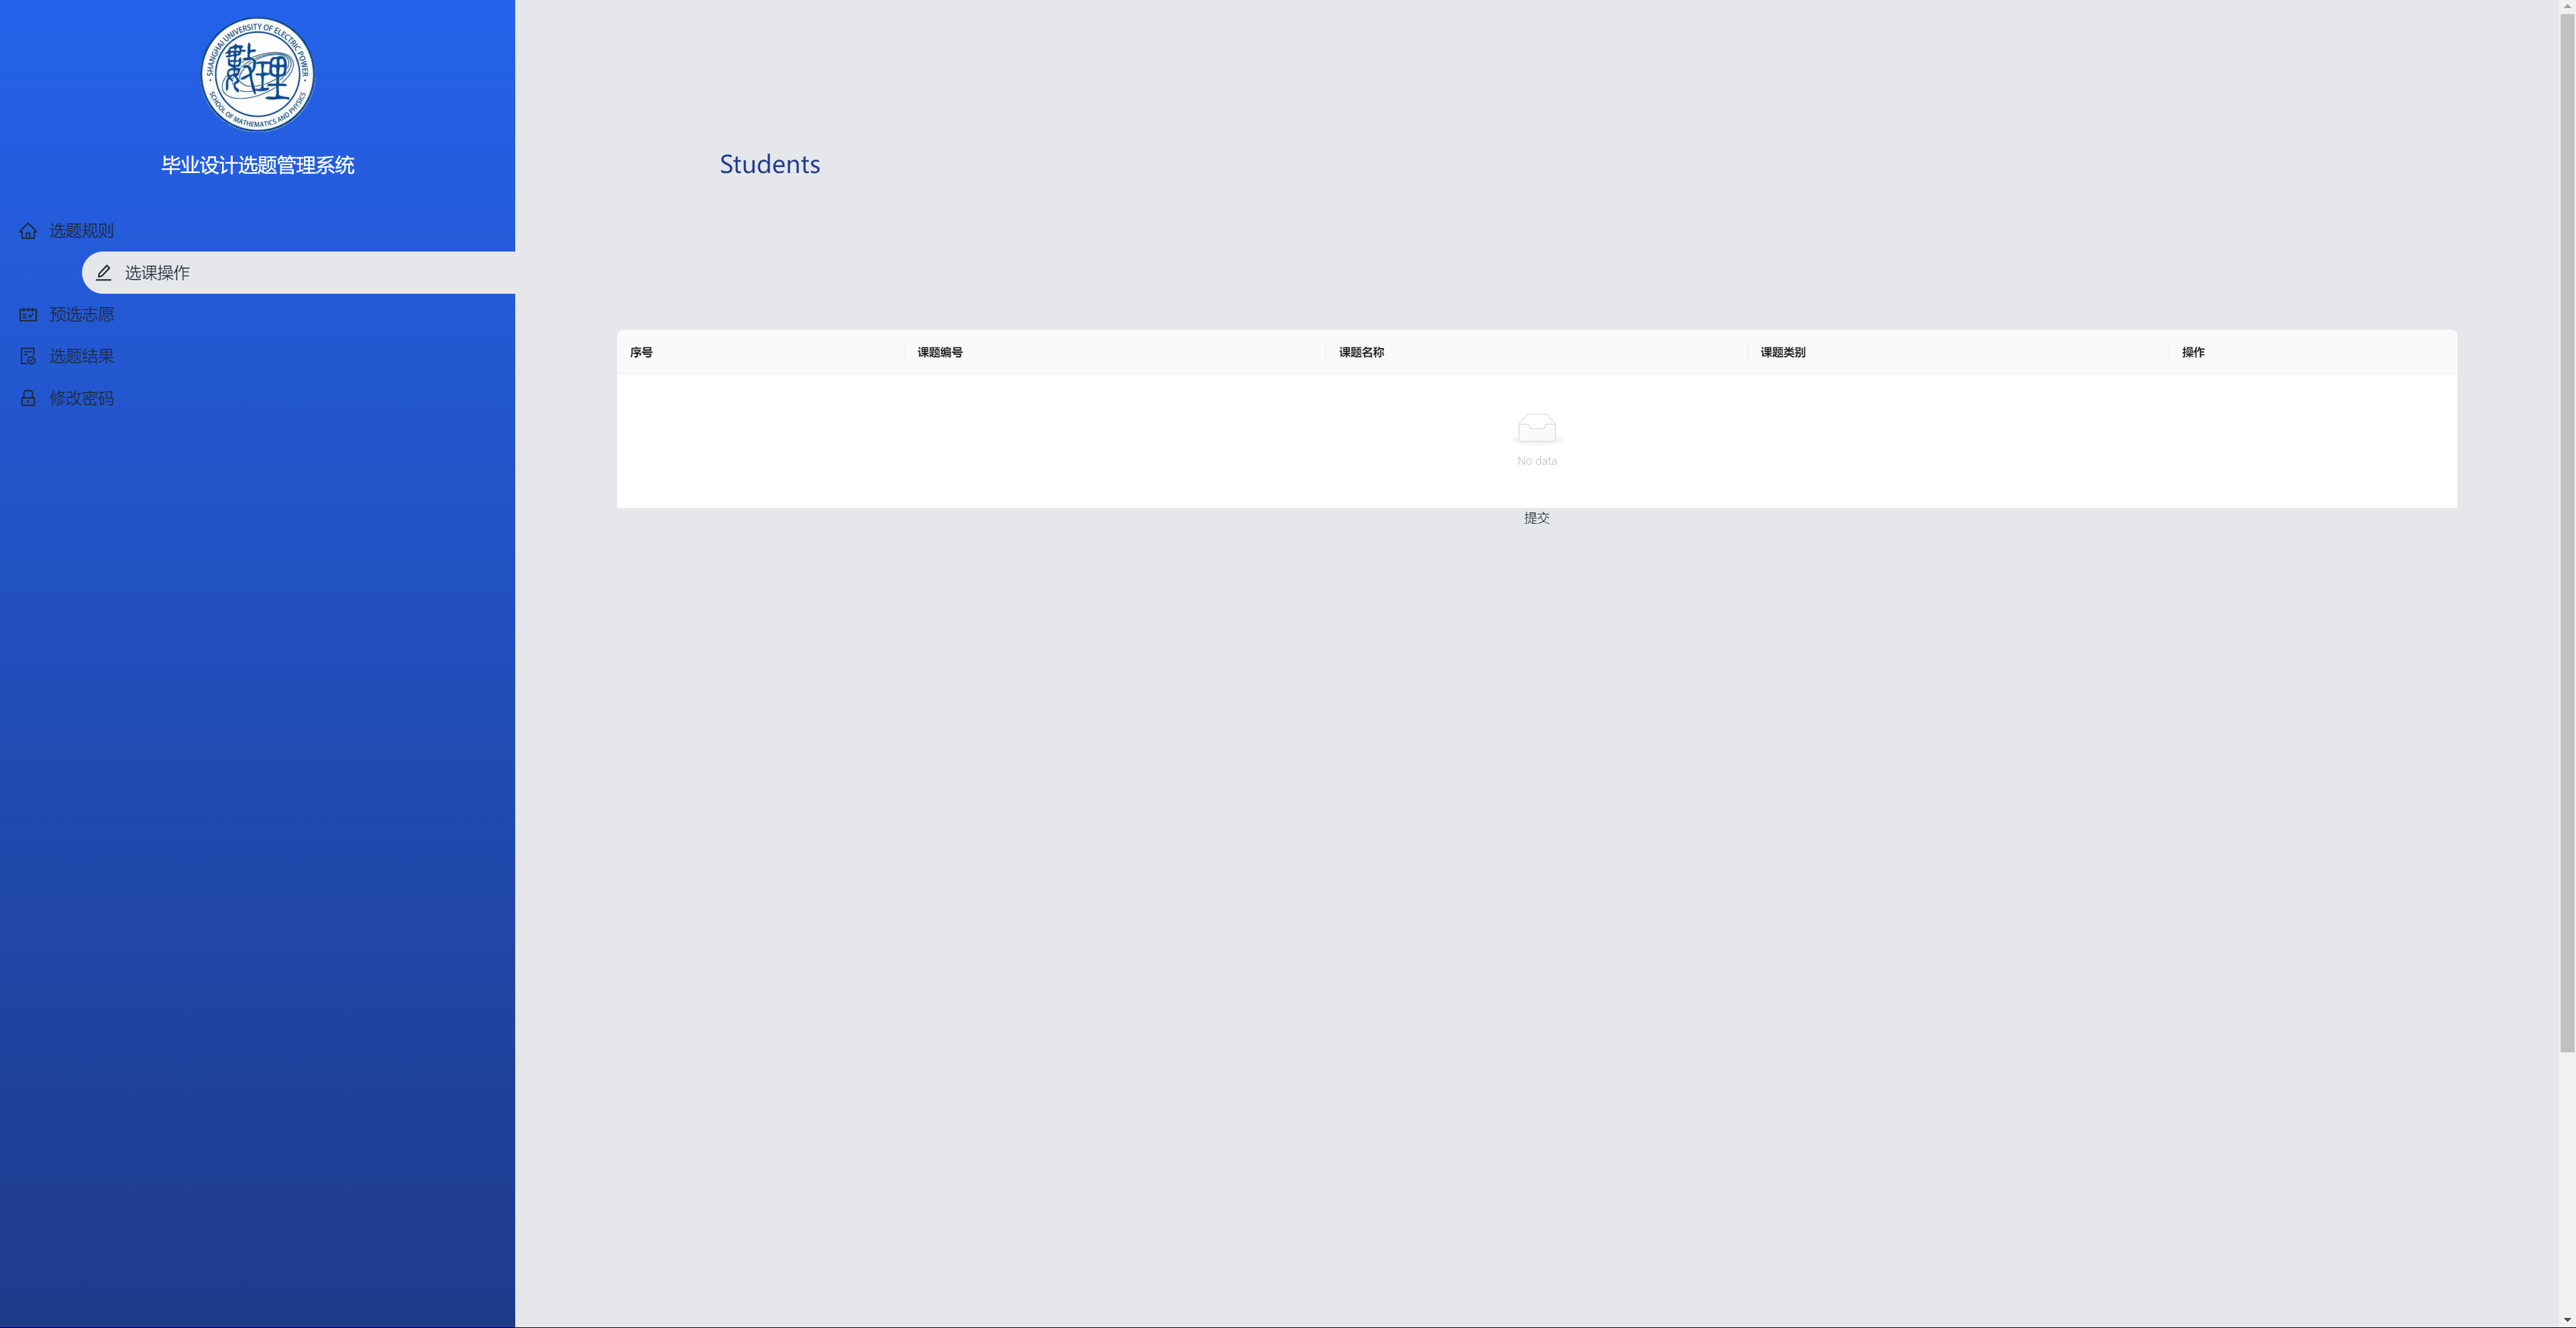
\includegraphics[width=1\textwidth]{学生端02.png}
    \caption{学生端-选课操作}
    \label{fig:student02}
\end{figure}

\clearpage

\subsubsection{预选志愿:}
在预选志愿界面,学生可以查看自己预选的第一到第四志愿,以及对应课题的信息。
\begin{figure}[h]
    \centering
    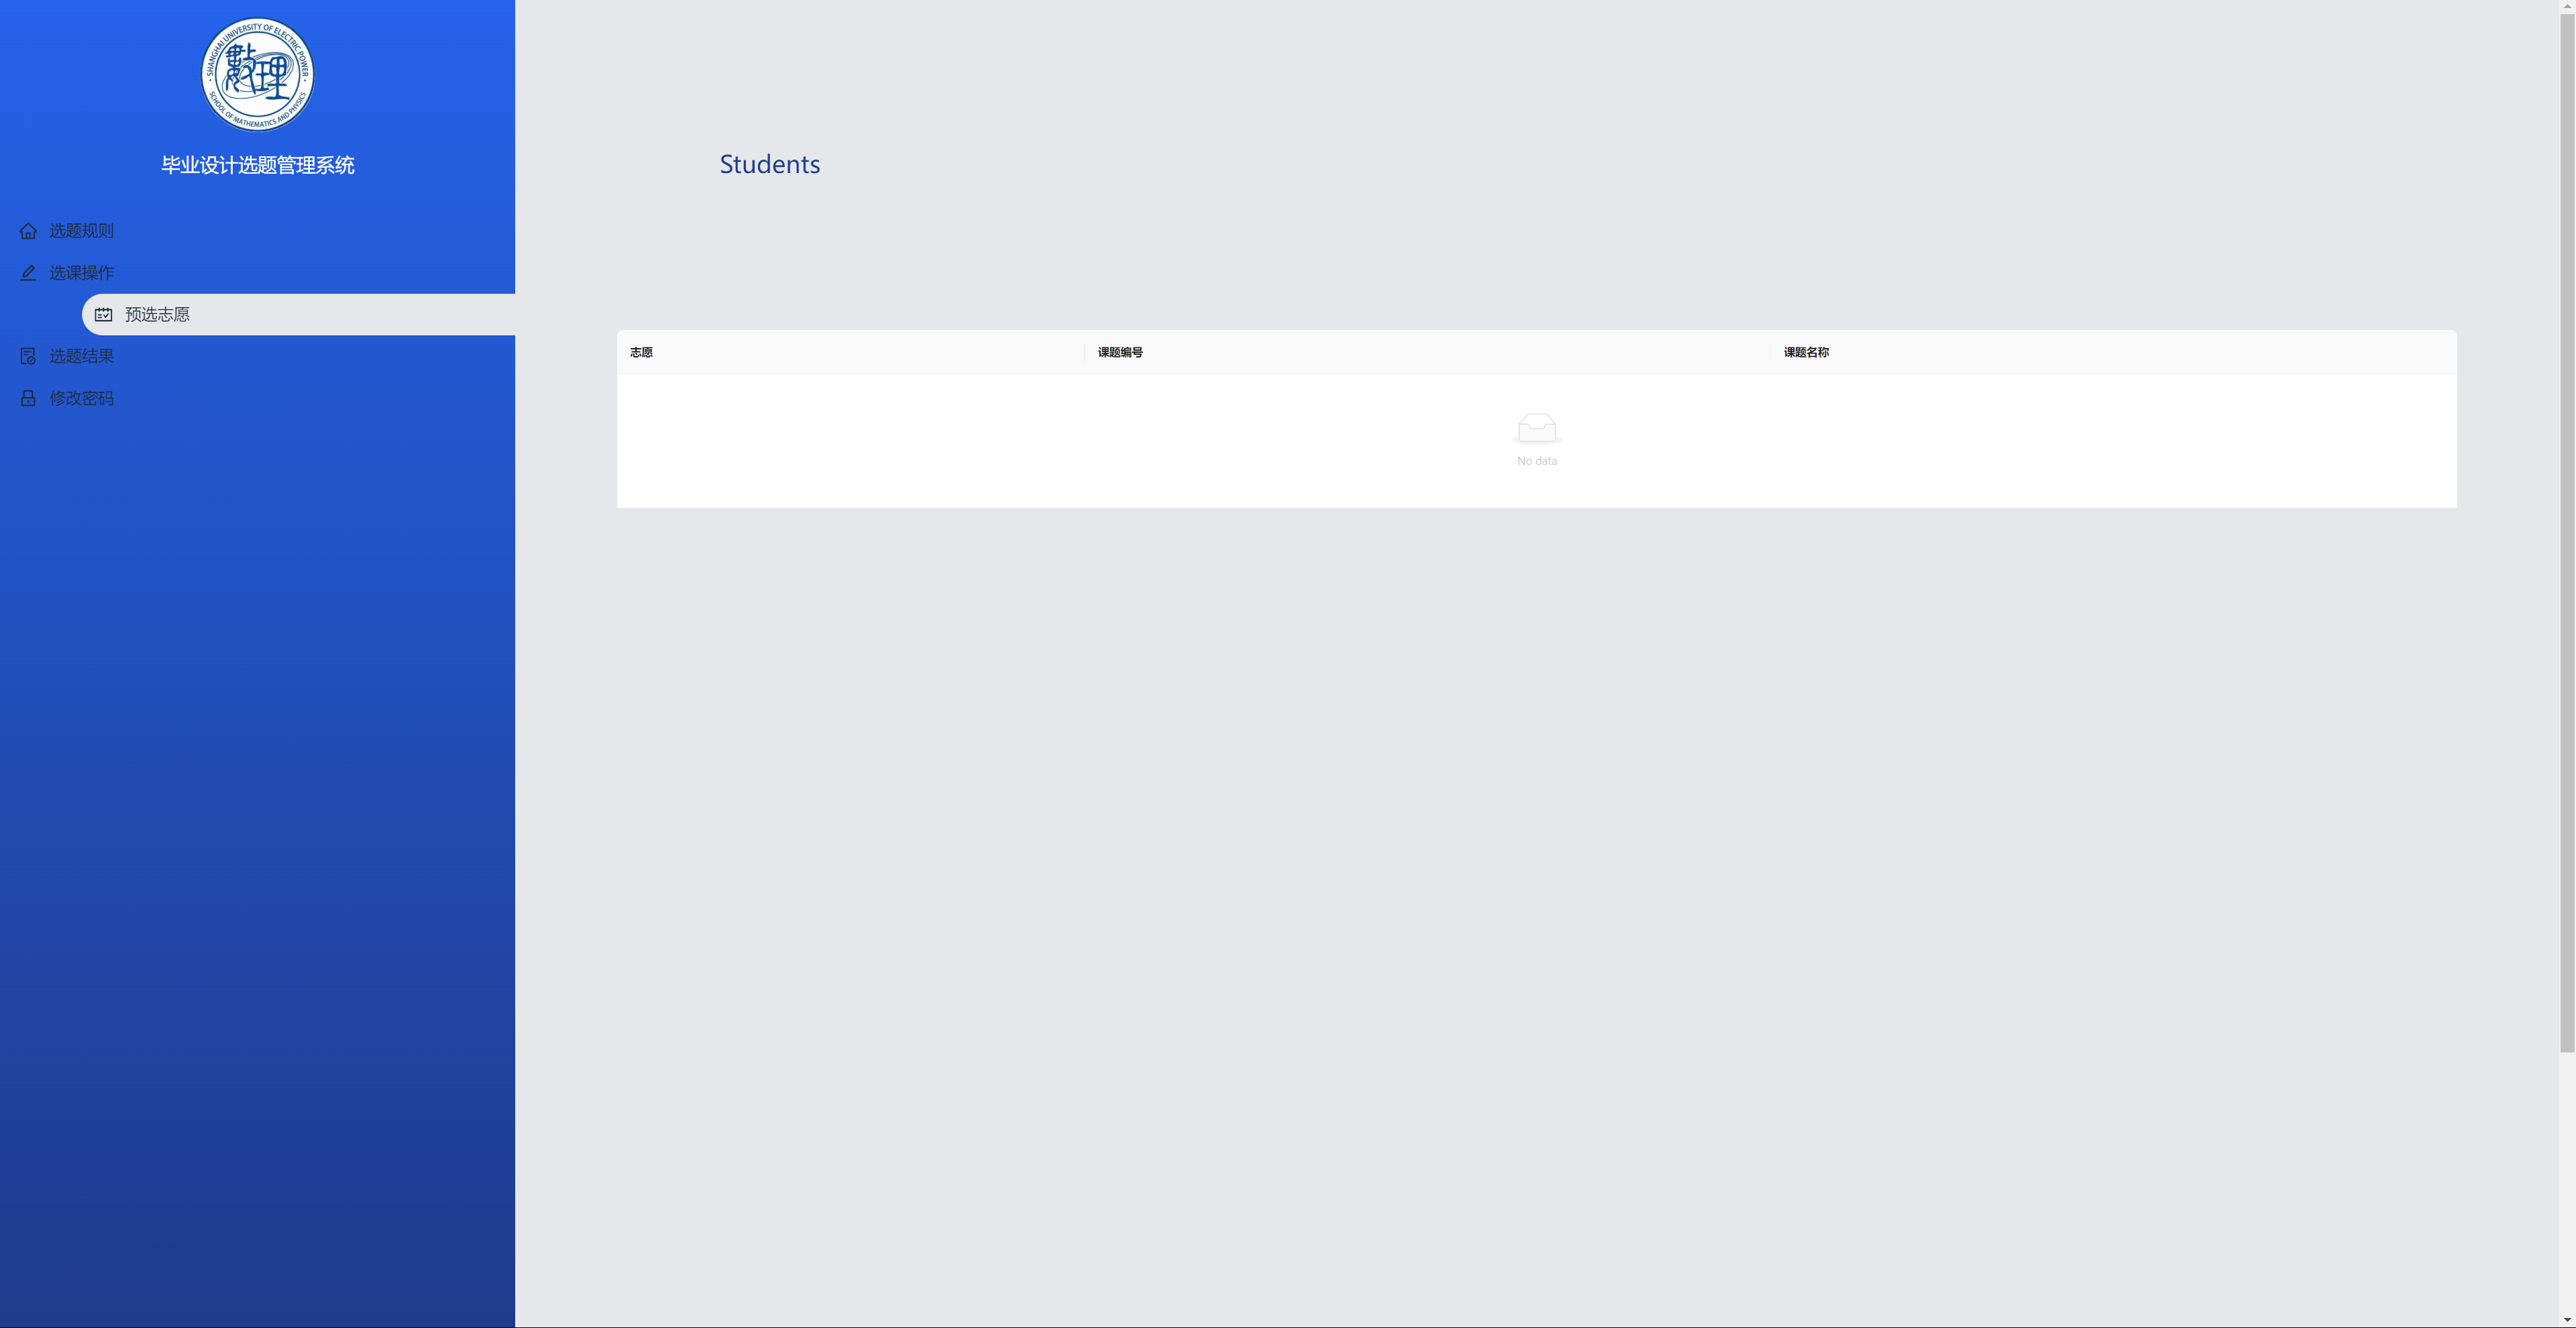
\includegraphics[width=1\textwidth]{学生端03.png}
    \caption{学生端-预选志愿}
    \label{fig:student03}
\end{figure}

\subsubsection{选题结果:}
在选题结果模块中,学生可以查看自己最后选择到的课题的课题编号、名称信息,
并且可以查看自己课题的指导老师。
\begin{figure}[h]
    \centering
    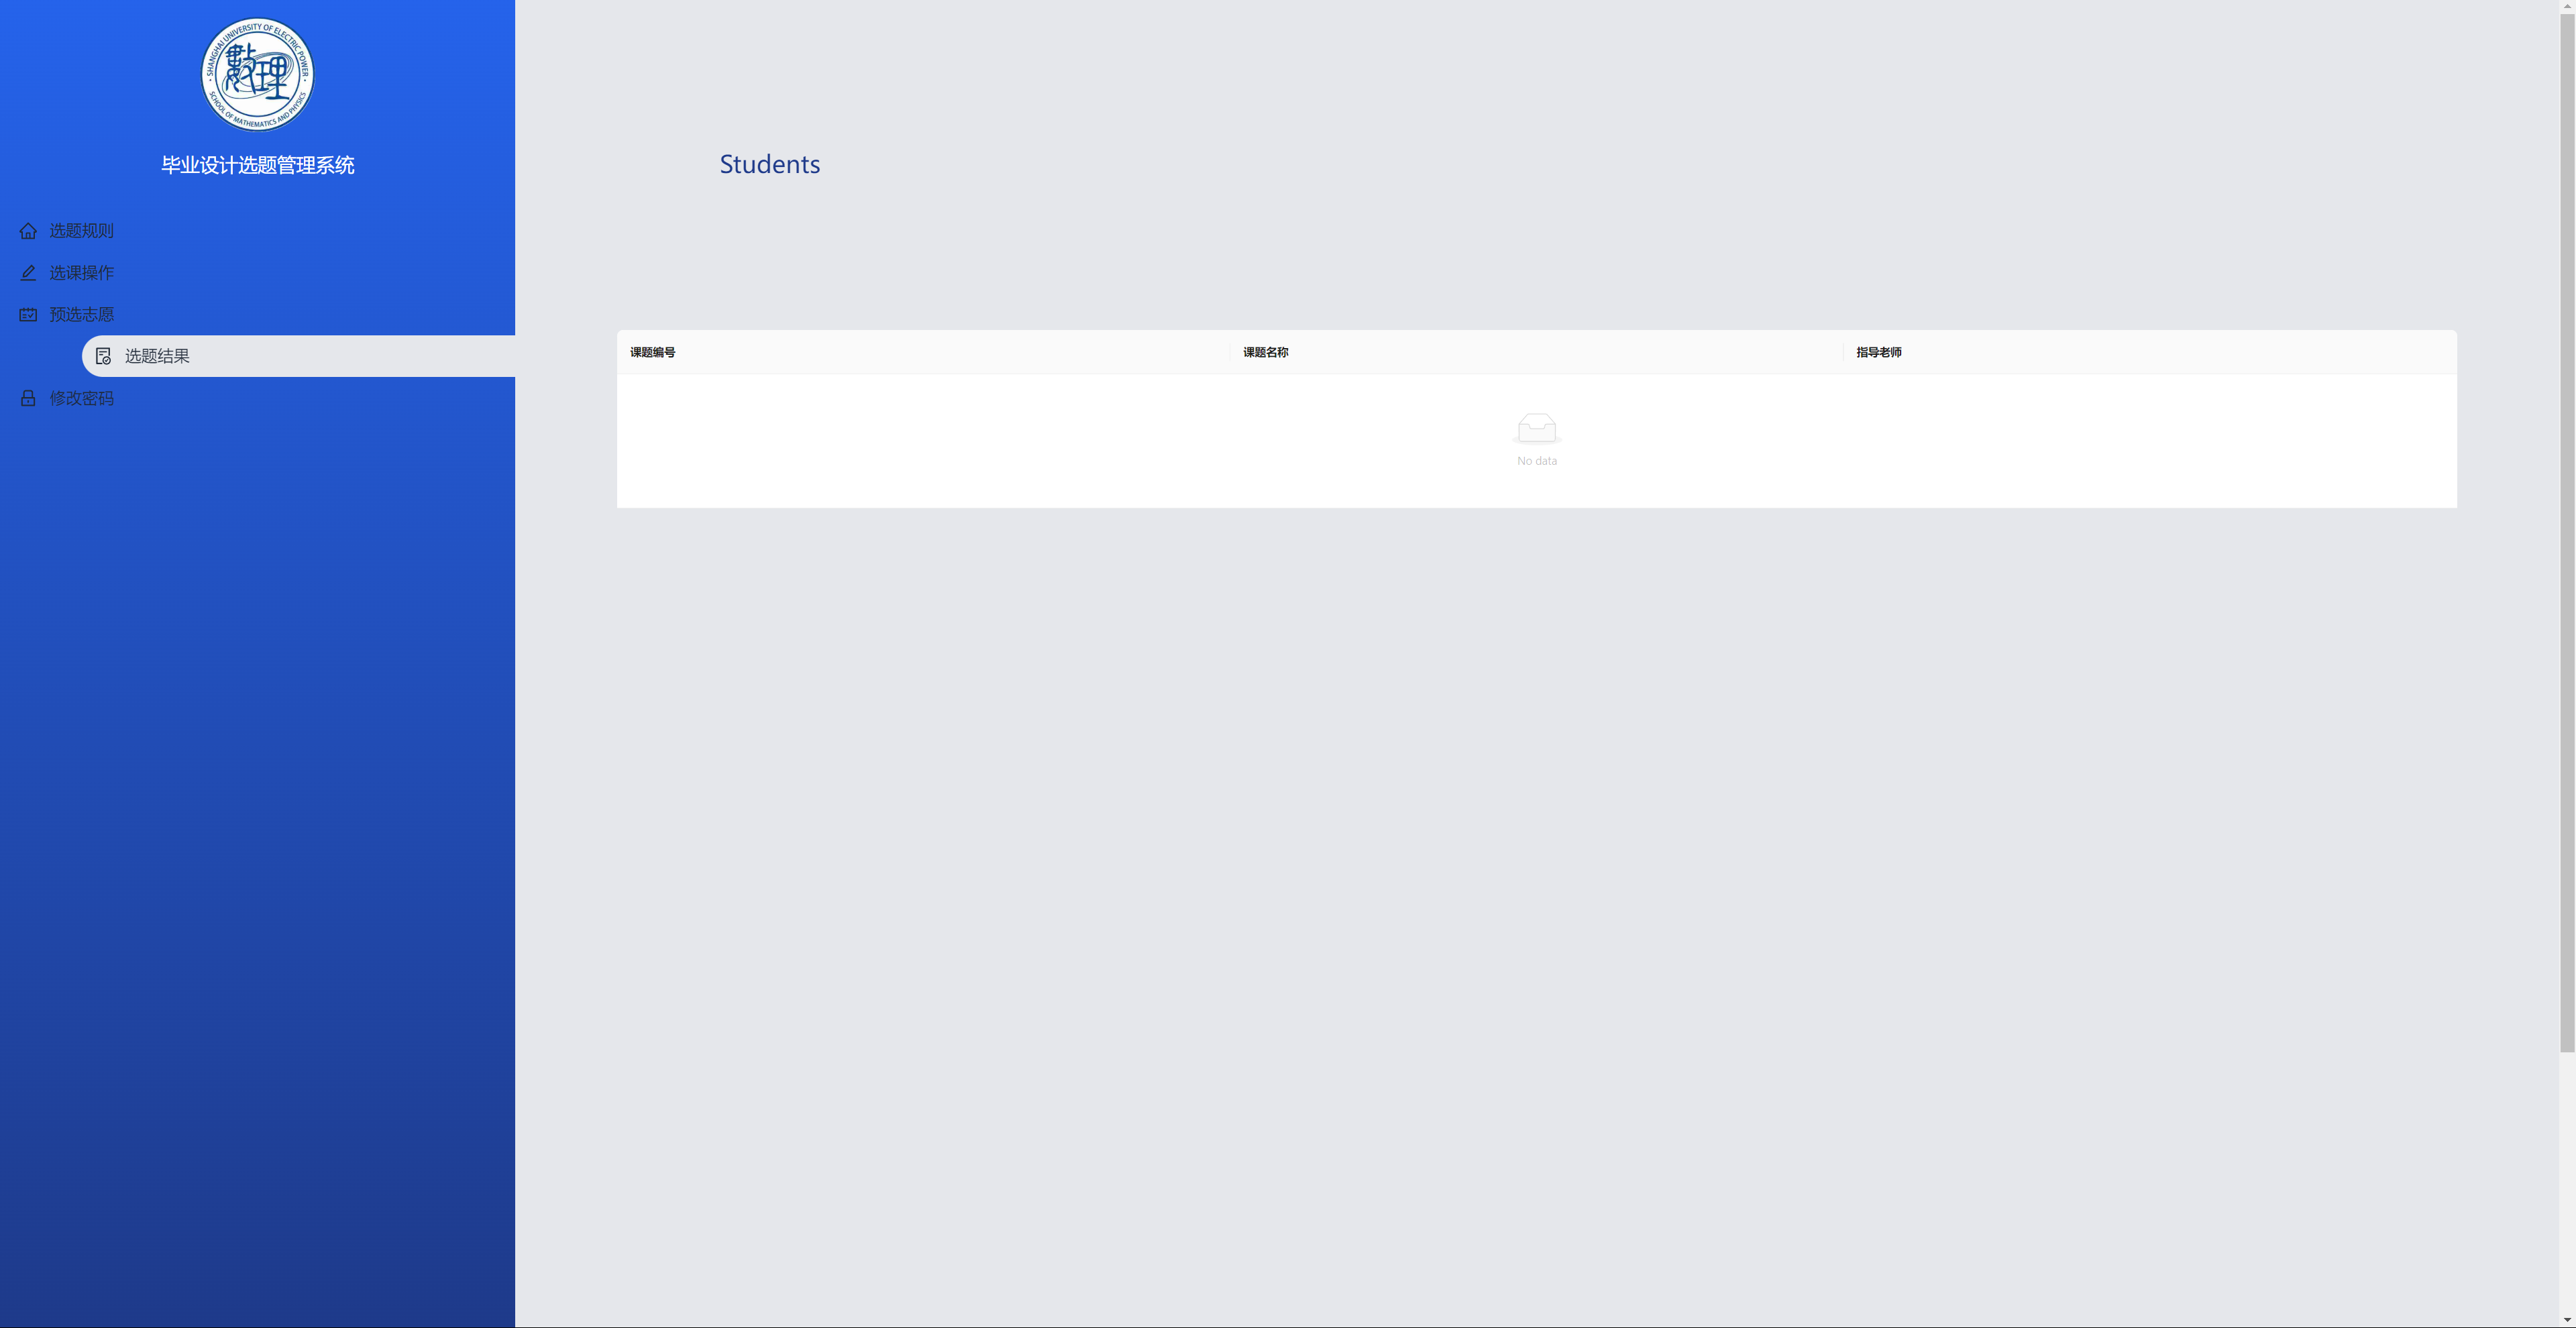
\includegraphics[width=1\textwidth]{学生端04.png}
    \caption{学生端-选题结果}
    \label{fig:student04}
\end{figure}

\clearpage

\subsubsection{修改密码:}
提供了学生更新密码的窗口。
\begin{figure}[ht]
    \centering
    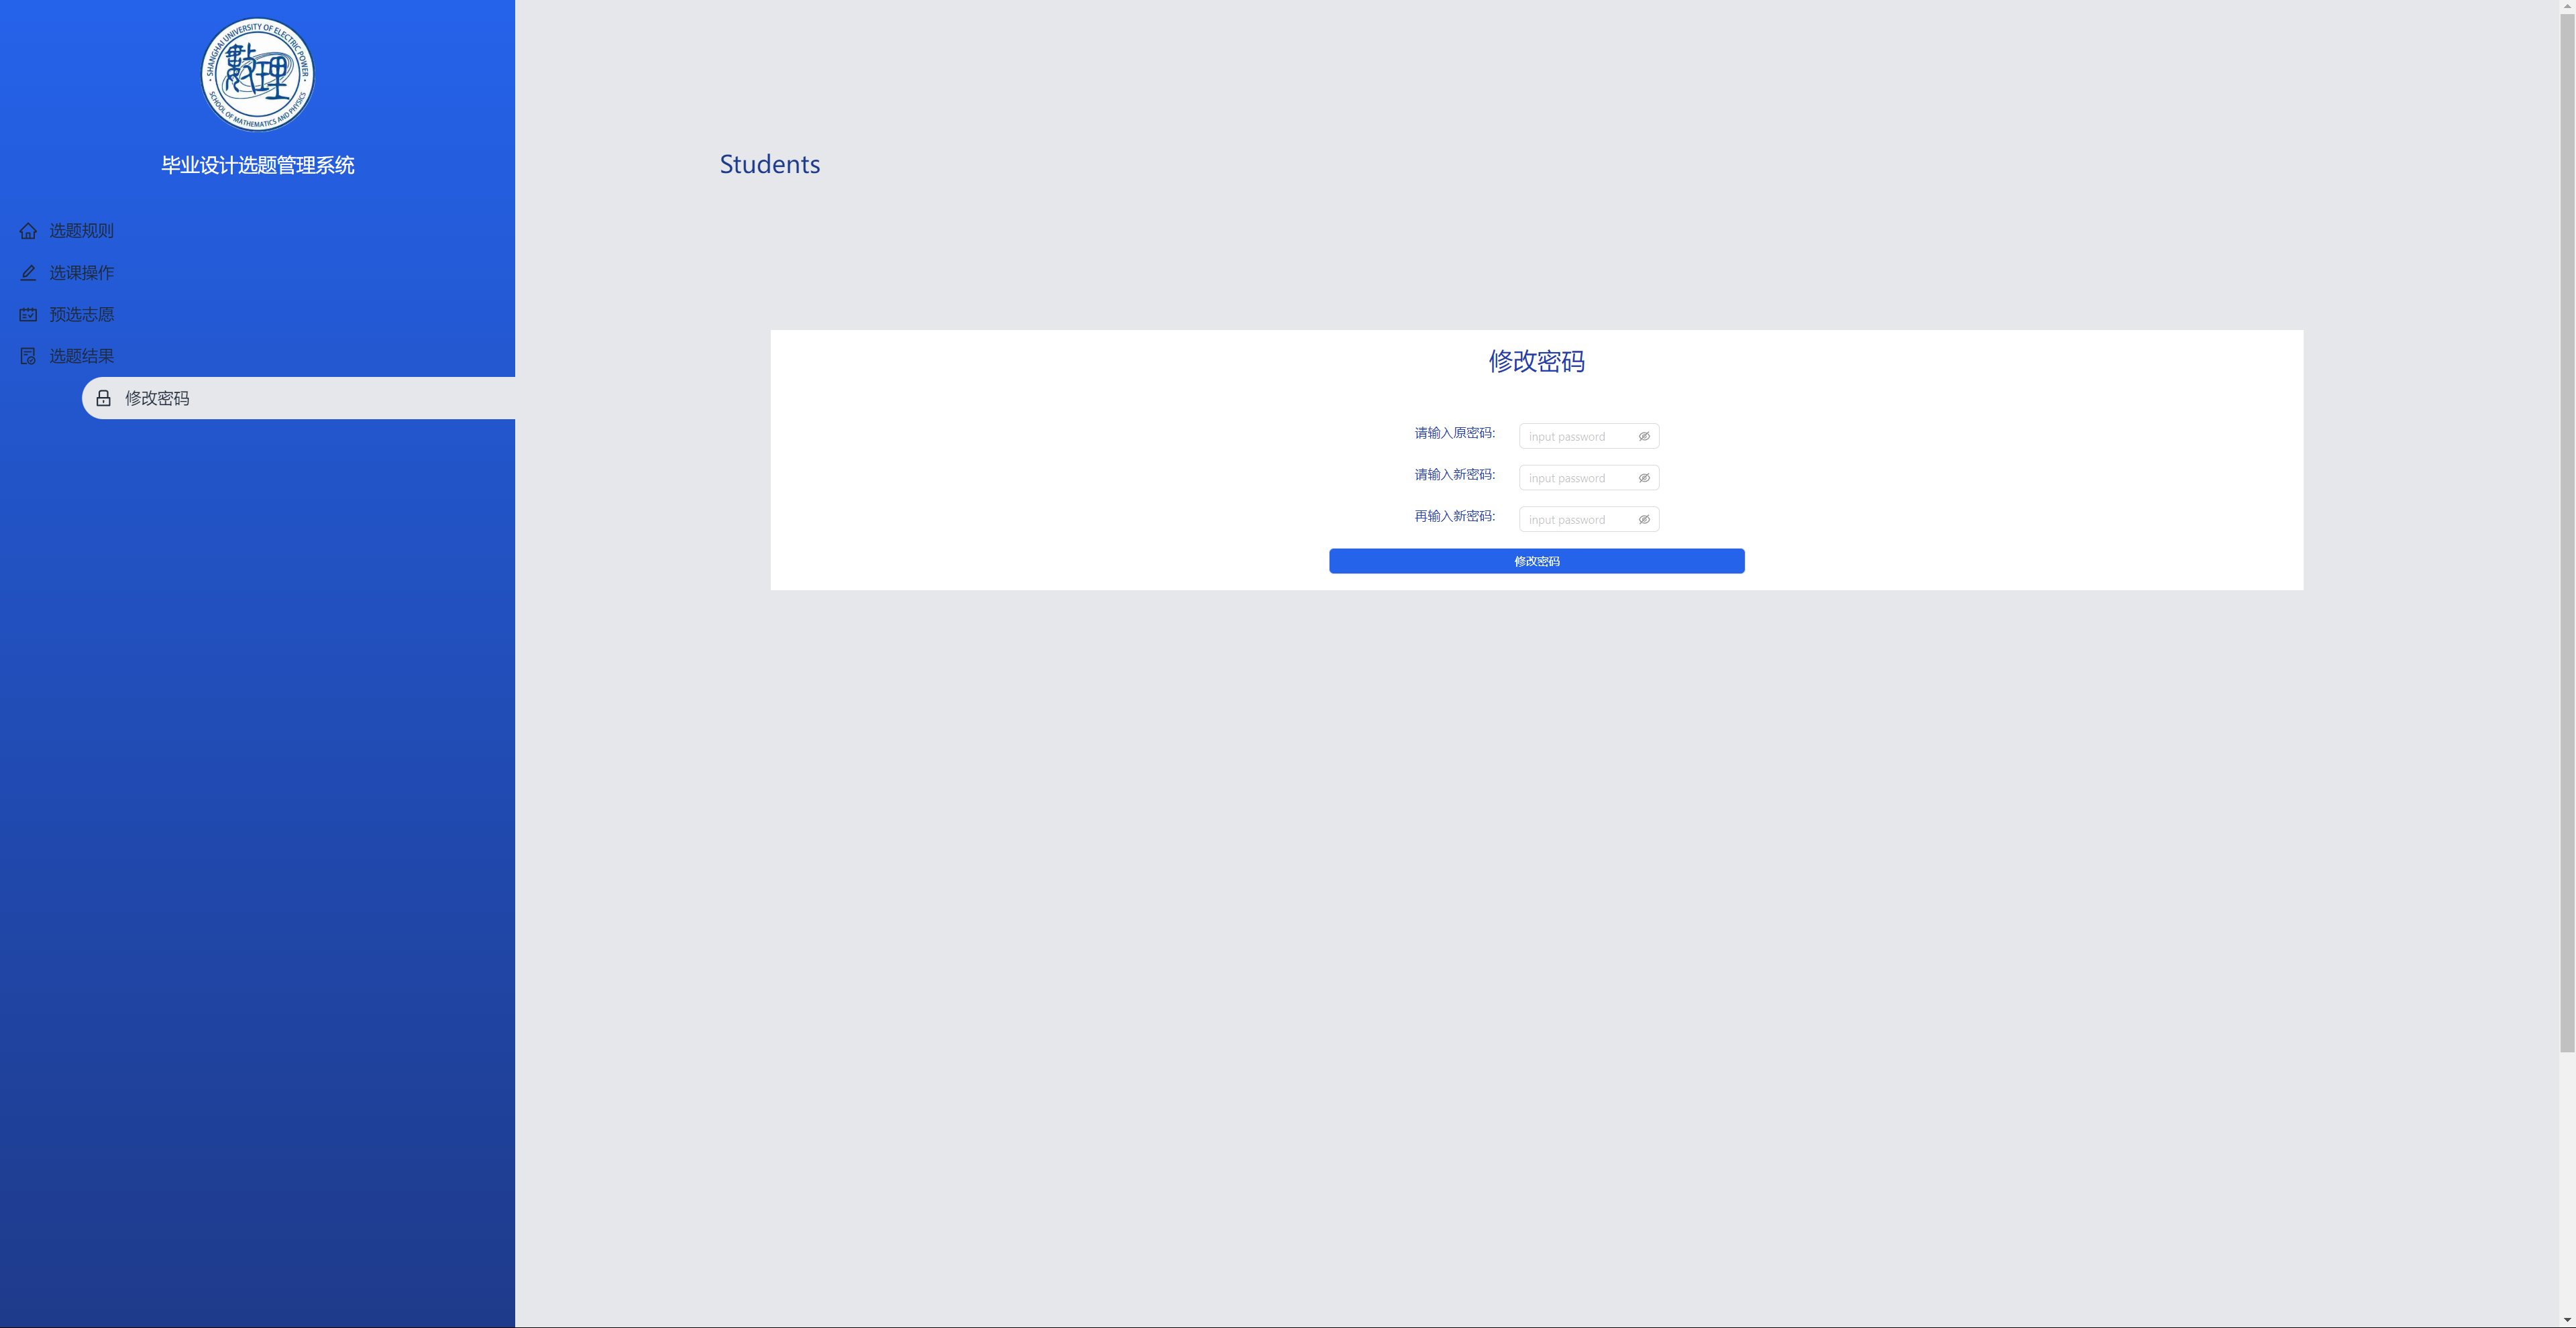
\includegraphics[width=1\textwidth]{学生端05.png}
    \caption{学生端-修改密码}
    \label{fig:student05}
\end{figure}


% =============================================
% Part 5 读后感
% =============================================
\section{必读材料读后感}
张辰星: 

大学的学习会让我们接触到各种各样许许多多的知识,但重要的乃是我们应该学会搜索汲取知识,真正的把这些知识化为己用。化为己用重点在要把知识系统性的理解掌握,系统性的讲出来又或者是系统性的做出来。在大学面对到的压力困难一定比你之前经历过的要大,但越是这样越应该有勇气有毅力的去面对它去解决它而不是逃避。


沈奕俊:


我认为这四篇文章带给我的不仅仅是为我学习CS做准备,更是对于我未来在计算机学习上的效率的提升,同时还是对于我为人处世的方式的升华。在这四篇文章里面我了解到了后续编程语言学习的障碍有多么艰巨和漫长,但我想我有信心在这条道路上一直走下去,并做好了面对困难付出大量时间精力的准备。这四篇文章为我在未来学习上的会遇到的问题提供了解决的方案、发出提问的地址、提问的语言艺术,而我也会牢记这些提问的要点,在提问前学会先尝试“rtfw”、“stfw”和“rtfsc”此类的准备和工作,再向他人提出的我问题,并清楚的说明我遇到的问题是什么,注释好我为我提出的问题已经做出了哪些尝试和努力,防止浪费大家的时间并确保我能及时的获得准确的帮助,避免成为“losers”中的一员。我也深刻的了解到了老师学长向我们这些还未入门的求学者推荐这几篇文章的用意,告知了我们前路的艰险以及为了通过所必须要付出的汗水与努力,同样也指引了我们方向、避免了我们走上许多不必要的弯路,在接下来的学习中使我们能够得到足够的磨炼成就自我,也让我们保持原有的道路而不是成为温室里的花朵或者在学习和以后的工作中成为问题宝宝。


包梵轩:

看完《提问的智慧》这一文章我感觉走进了一个新的领域,就以前的提问方式,自己对问题的理解程度不清楚,对问题的解决方法不清晰,只知道“百度”,问同学等一些不专业的方式,读完这篇文章之后,我清楚的了解到提问的步骤有前后中之分,提问前应该先尽自己努力去尝试自行解决问题,提问时应注意选择正确的论坛,写有意义的标题内容,语言表达也要得体,以及提问时也是一个沟通的过程而绝非低声下气,而看到RTFM和STFW这种具有幽默性质的网络文化用语时,也更激发了我学习的兴趣,更让我学会了如何做一个有智慧的问题提出者。
\end{document}
